\chapter{Inklusion im Kindergarten}

\section{Warum Inklusion?}
\label{sec:Why}
Es folgen eine Reihe ausgewählter Begründungen, die zeigen, welchen Nutzen der Kindergarten verspricht, dessen Selbstverständnis es ist keine Türen der Ausgrenzung zu haben und inklusive Erziehungs- und Bildungsarbeit zu leisten. 

\subsection{Leben in einer Art 'Parallelgesellschaft'}
Erhardt und Grüber (2011, 36) verweisen auf das Argument, dass Menschen mit Behinderung nicht länger ihr Leben in Sondereinrichtungen vollziehen wollen, sondern dort, wo alle anderen auch sind. Die Forderung der uneingeschränkten Teilhabe impliziert demnach das Beenden der Segregation, von der vor allem die Personengruppe mit schwer geistiger oder Mehrfachbehinderung oder die Menschen mit psychischen Erkrankungen betroffen sind. Wenn über Inklusion gesprochen und im Zusammenhang damit die uneingeschränkte Teilhabe aller Menschen gefordert wird, so wird oft dem Gedanken gefolgt, dass es eine 'allgemeine Welt' gibt, an der alle mit Ausnahme der Menschen mit geistiger Behinderung teilhaben können. Dabei unberücksichtigt bleibt die Tatsache, dass es auf verschiedensten Ebenen Zugangsbeschränkungen gibt, die Teil der Gesellschaft sind und von dieser auch nicht infrage gestellt werden. Dazu zählen zum Beispiel Vereine, Subkulturen oder die Kantine des Bundestages. Der Unterschied zu Menschen mit Behinderung besteht darin, dass sich deren Teilhabe an zentralen Lebensbereichen in einem eigens für sie geschaffenen Subsystem abspielt -- in einer Parallelwelt.
Gesetz den Fall ein Kind mit einer schweren Behinderung wird geboren, so wächst es entweder in seiner Herkunftsfamilie auf oder ist in einer großen Einrichtung, einer so genannten Komplexeinrichtung, untergebracht, welche sich zumeist fern von Ballungszentren an Stadtrandgebieten oder auf dem Lande befinden. Auch wenn das Kind  innerhalb seiner Familie aufwächst, spielt sich zumeist sein gesamtes außerhäusliches Leben in Einrichtungen der Behindertenhilfe ab. Diese hier aufgezeigte deutsche Entwicklung, die sich im Zuge der Ambulatisierungsbewegung allmählich beginnt zu ändern, hatte zur Folge, dass Menschen mit geistiger Behinderung viele Jahre nicht zum Straßenbild gehörten, so dass sie schon deswegen nicht inkludiert werden und eine sozial geachtete Rolle einnehmen konnten, weil es keine Berührungspunkte und Begegnung gibt. Durch das hoch differenzierte Behindertenhilfssystem und das Verwahren in psychiatrischen Einrichtungen ist eine deutsche Kultur begünstigt worden, in der Menschen mit Behinderung nicht zum normalen Umgang gehören und deshalb als befremdlich empfunden werden können.
So beschreiben Erhardt und Grüber (2011, 10), dass sowohl Menschen mit als auch Menschen ohne Behinderung aufgrund ihrer mangelnden Kontakte ungeübt sind in der Kontaktaufnahme, weshalb es auf der einen Seite die Ängste und Zurückhaltung der Menschen ohne Behinderung ernst zu nehmen gilt und auf der anderen Seite gleichzeitig Begegnung und gemeinsame Lebenswelten zu fördern sind. Die beste Voraussetzung dafür, dass gemeinsame Lebenswelten in Zukunft selbstverständlich werden und ein „toleranteres und wärmeres gesellschaftliches Klima“ (Haug 2011, 42) entstehen kann, ist das gemeinsame Aufwachsen aller Kinder. 

\subsection{Die UN-Behindertenrechtskonvention}
\label{sec:BRK}
Dass sich das Leben von Menschen mit Behinderungen nicht in Sondersystemen, sondern so weit wie möglich innerhalb der allgemeinen Lebenswelt abspielt, ist nicht nur der Wunsch von Behindertenverbänden, sondern ist durch die Unterzeichnung der UN-Behindertenrechtskonvention rechtskräftig. Wie auch die Kinderrechtskonvention ist die \emph{„UN-Behindertenkonvention über die Rechte von Menschen mit Behinderung“} laut Albers (2011, 26 f.) ein völkerrechtliches Abkommen. Die Mitgliedsstaaten verpflichten sich durch Unterzeichnung die im Völkervertrag getroffenen Bestimmungen in ihr nationales Rechtssystem umzusetzen. Die Konvention wurde im Dezember 2006 von der Generalversammlung der vereinten Nationen verabschiedet. Im März des Folgejahres wurde sie von Deutschland unterzeichnet, im Dezember 2008 vom Deutschen Bundestag und Bundesrat ratifiziert und ist seit 24.03.2009 in deutsches Recht umzusetzen. Das heißt, dass bestehende Gesetze überprüft und den Vorgaben der Behindertenrechtskonvention angepasst werden müssen. Damit liegt laut Klein (2011, 13) für die Arbeit im Kindergarten ein verbindlicher Handlungsrahmen vor. Bildungs- und Sozialpolitiker sind herausgefordert, Rahmenbedingungen für eine gelingende inklusive Praxis zu schaffen. Er (2011, 91) betont, dass angesichts der Größe der Aufgabe das Schaffen geeigneter Rahmenbedingungen (vgl. Kapitel~\ref{sec:Wie}) nur schrittweise erfolgen kann. Inwieweit inklusive Bildung und Erziehung von Kindern mit Behinderungen tatsächlich verwirklicht wird, bleibt laut ihm (2011, 13) eine offene Frage. Die Umsetzung der Konvention hängt vom politischen Willen und der konkreten Bildungspolitik von Regierungen ab, und davon, wie lange es dauert, bis Inhalte und Ziele der Konvention in den Köpfen und Herzen der politischen Akteure auf Bundes-, Landes- und kommunaler Ebene angekommen sind. „Es muss sich aus dem sozialen Bewusstsein der Menschen entwickeln“, schreibt Klein (2011, 13). 

Nach Wunder (2009) werden in der UN-Konvention keine Sonderrechte zugesprochen, stattdessen werden aus der Perspektive der Menschen mit Behinderung die universell geltenden Menschenrechte konkretisiert und spezifiziert, so dass diese Personengruppe, die einen erschwerten Zugang zu Grundrechten hat beziehungsweise vermehrt Gefährdungen ausgesetzt ist, unter den notwendigen Menschenrechtsschutz gestellt ist, mit dem Ziel ihre volle gesellschaftliche Teilhabe und Chancengerechtigkeit weltweit zu fördern. Das Übereinkommen würdigt laut Klein (2010) Behinderung als Teil der Vielfalt menschlichen Lebens und überwindet damit das vorherrschende Prinzip der Wohltätigkeit und Fürsorge. Inklusion ist demnach keine wählbare Idee mehr, sondern ein Menschenrecht, das auf allen Ebenen umzusetzen ist. In Artikel 24 der Behindertenrechtskonvention wird das inklusive Recht auf Bildung betont: „States Parties recognize the rights of persons with disabilities to education. With the view to realizing this right without dicrimination and on the basis of equal opportunity, States Parties shall ensure an inclusive education system at all levels and lifelong learning [...]“ (Haug 2011, 38). An dieser Stelle wird in Originalsprache zitiert, da in der deutschsprachigen Übersetzung zahlreiche Begriffe von emanzipatorischen Wert laut Wocken (2011) durch bedeutungsschwächere Begriffe übersetzt worden sind. Das Recht auf inklusive Bildung wurde als Recht auf Bildung abgestuft, dieses Beispiel stützt seine These über die 'Entkernung' der Behindertenrechtskonvention, die durch die deutsche Übersetzung stattgefunden hat. „Bei der verkürzten Redewendung 'Recht auf Bildung' handelt es sich nicht um ein unschuldiges und harmloses Sprachspiel, sondern um die bewusste und durchaus destruktive Absicht, den Auftrag zur Entwicklung eines inklusiven Schulsystems substantiell zu unterlaufen [...]“ (Wocken 2011).

\subsection{Wohnortnahe Betreuung als Ressource}
Die Freiburger Projektgruppe (1993, 21-24) benennt als weitere Begründung für inklusive Kindergärten begünstigende psychosoziale Faktoren, die sich aus der Nähe der öffentlichen Betreuung zum Wohnort der Familie ergeben. Für die wenigsten Kinder in einer unterstützungsbedürftigen Lage kann der Kindergartenbesuch 'vor der Haustür' verwirklicht werden. Obwohl es mittlerweile vielerorts, vor allem in größeren Städten, Möglichkeiten der gemeinsamen Betreuung gibt, ist der Besuch einer solchen Einrichtung für viele Familien mit weiten Anfahrtswegen verbunden. 

Bei Betrachtung der Entwicklungsschritte eines Kindes, fällt auf, dass sich das Kind zuerst seine unmittelbare familiäre Umgebung erschließt und dann seinen Erfahrungshorizont auf soziale Bezüge außerhalb der Familie erweitert, wie Nachbarschaft, Kindergarten, Spielgruppe oder Gemeinde. Wenn der wohnortnahe Kindergarten die 'Tore für sämtliche Kinderwelten' öffnet, kann das Kind und mit ihm seine Familie im Laufe der Kindergartenzeit in ein soziales Netz hinein wachsen, dessen Aufbau als Meilenstein in der kindlichen Entwicklung angesehen wird. 
Somit wird die Teilhabe laut Jerg (2011, 56) zur Voraussetzung, um überhaupt eine Beteiligungskultur in Bezug auf das unmittelbare soziale Umfeld aufbauen zu können. Der Aufbau einer Beteiligungskultur besteht darin, dass Kinder mit besonderem Unterstützungsbedarf in die Lage versetzt werden, die Rolle des Spielpartners zu übernehmen, wodurch sie für andere bedeutsam werden. Das wiederum ist an die Bedingung geknüpft, dass Beziehungen zu Spielgefährten und Freunden gepflegt und erhalten werden können, was voraussetzt, dass die dafür notwendige Zeit zur Verfügung steht und das Kind nicht aus seinen normalen Lebensvollzügen heraus genommen wird.
Mit der Teilhabe wächst die so genannte „Teilgabe“, worunter Jerg (2011, 57) versteht, dass Kinder mit Unterstützungsbedarf Möglichkeiten haben sich und ihre Fähigkeiten einzubringen und dafür Anerkennung zu erhalten. 
Wenn das Kind nun in einen Kindergarten geht, der in einem anderen Stadtteil liegt, gehen dadurch wichtige soziale Entwicklungsbedingungen in der Nachbarschaft verloren. das gilt nicht nur für das Kind, sondern auch für die Familie, für welche soziale Beziehungen im Lebensumfeld ebenfalls wichtige Ressourcen darstellen. Durch die Teilhabe ihrer Kinder an regulären Lebensvollzügen eines öffentlichen Kindergartens sind die Chancen erhöht, dass durch wohnortnahe Alltagsbegegnungen sowohl das Kind als auch die Familie Kontakte knüpfen können und die betroffenen Eltern soziale Unterstützung erfahren. Damit sind wichtige Voraussetzungen geschaffen, dass sich die Familie die genannten Ressourcen erschließen kann und vor sozialer Ausgrenzung geschützt ist. 

\subsection{Die Verschiedenheit der Kinder ist eine soziale Tatsache}\label{sec:heterogenität}
Nach Sander (2004, 242) setzt Inklusion voraus, die Individualität aller Kinder anzuerkennen und als erzieherische Herausforderung zu begreifen. Inklusion basiert auf der grundlegenden Erkenntnis, dass alle Menschen verschieden sind. Auch unter Menschen ohne Behinderung gibt es Unterschiede. Mit Hilfe der Forschungsergebnisse von Remo Largo (2011, 16, 25), der zwischen 1954 und 1998 in Längsschnittstudien das Wachstum und die Entwicklung von 800 Kindern untersucht hat, kann gezeigt werden, dass das Ausmaß der Vielfalt bei Kindern so groß ist, dass alle nicht individualisierten Angebote zu scheitern drohen. Jedes Kind hat seine eigenen Stärken und Schwächen und ein eigenes Entwicklungstempo, diese Merkmale werden es bis ins Erwachsenenalter begleiten. Im Laufe der Entwicklung nehmen die Unterschiede immer mehr zu. 

Laut Largo (2011, 25) ist es nicht so, dass Unterschiede bei Kindern nicht bemerkt werden würden. Dass Kinder eine unterschiedliche Augen- oder Haarfarbe, Körpergröße oder ein unterschiedliches Gewicht haben, fällt ins Auge. Weniger selbstverständlich ist jedoch die Variabilität von Unterschieden, die man nicht sogleich sehen kann, wie Sozialverhalten oder geistige Fähigkeiten. Die Variabilität des Sozialverhaltens oder der geistigen Fähigkeiten ist bei normal entwickelten Kindern sogar wesentlich ausgeprägter als bei phänotypischen Merkmalen. Die Variationsbreite einiger Merkmale wird folgend illustriert, wodurch laut Largo (2011, 25) gezeigt werden kann, dass „die Vielfalt ein durchgehendes Merkmal der kindlichen Entwicklung ist“. Nach Largo (2011, 29 f.) beginnen die meisten Kinder die ersten drei Wörter zwischen ihrem zwölften und 18. Lebensmonat zu sprechen, manche aber auch erst zwischen dem 21. und 33. Lebensmonat. Zwischen Früh- und Spätentwickler besteht somit ein Unterschied von 18 Monaten. Zwei-Wort-Sätze beginnen einige bereits mit 13 bis 18 Monaten, die meisten zwischen 18 und 24 Monaten zu bilden. Einige wenige, in den meisten Fällen Jungen, bilden Zwei-Wort-Sätze erst nach dem dritten Lebensjahr. Hierbei beträgt der Unterschied mehr als zwei Jahre. Die Variationsbreite im Hinblick auf geistige Fähigkeiten wie Lesen und Rechnen ist ebenfalls groß. Manche Kinder lernen bereits im Kindergartenalter lesen, sie bringen es sich selbst bei. Andere Kinder erlangen die Fähigkeit zu lesen erst gegen Ende des ersten Schuljahres. In einer ersten Schulklasse gibt es Kinder, deren rechnerisches Verständnis einem Entwicklungsstand von fünfeinhalb bis sechseinhalb entspricht, das Verständnis anderer entspricht dem Entwicklungsstand von Acht- bis Achteinhalbjährigen. Auch in Bezug auf das Bindungsverhalten lassen sich laut Largo (2011, 43) große Unterschiede fest machen. Manche Kinder, vorwiegend Mädchen, sind bereits mit zwei bis drei Jahren emotional selbstständig, so dass sie sich in öffentlicher Betreuung wohl fühlen, andere wiederum zeigen mit fünf Jahren immer noch großen Widerwillen einen halben Tag, getrennt von der Mutter, im Kindergarten zu verbringen. Entgegen der Meinung vieler Fachleute weist Largo (2011, 124) darauf hin, dass die Bindungsbereitschaft wie jede andere Verhaltenseigenschaft von Kind zu Kind variiert. Gleichaltrige Kinder sind unterschiedlich stark gebunden und emotional unterschiedlich abhängig von ihren Bezugspersonen. 

Nach Aussage von Largo (2011, 15) gilt, je besser es Pädagogen gelingt, sich auf die individuellen Bedürfnisse und Eigenheiten der Kinder einzustellen, desto besser werden sich diese entwickeln, desto geringer wird der erzieherische Aufwand sein und desto weniger Verhaltensauffälligkeiten werden die Kinder entwickeln, weil sie weder unter- noch überfordert worden.   

Ziel des inklusiven Ansatzes ist es die Unterschiede nicht als Problem wahrzunehmen, sondern ihnen mit Wertschätzung zu begegnen, Vielfalt gar als Motor für Entwicklung zu nutzen. Das Problemverständnis wird in dem von Görannson (2011, 17 f.) illustrierten Fallbeispiel des Mädchens Anna als das entscheidende handlungsleitende Motiv dargestellt, wie mit der Verschiedenheit der Kinder in der Praxis umgegangen wird und welche Maßnahmen ergriffen werden, um Probleme abzumildern oder zu lösen. Göransson formuliert die Frage, warum sich Anna die meiste Zeit im Kindergarten mit Begeisterung an den Spiel- und Lerntätigkeiten beteiligt. Die Autorin gibt als Antwort, dass Annas aktive Teilnahme wohl kaum an außergewöhnlichen Fähigkeiten liegen mag, als vielmehr daran, dass die Aktivitäten so entwickelt wurden, dass diese ihr Interesse wecken und deshalb für sie wie auch für die meisten anderen Kinder in der Gruppe passend erlebt werden. Wenn wir Anna aber nun einen selbst erfundenen Peter gegenüber stellen, der häufig allein in einer Ecke des Raumes sitzt und wenig Eigeninitiative ergreift, an Aktivitäten teilzunehmen oder Kontakt zu anderen Kindern herzustellen, würden wir dann dem soeben favorisierten Erklärungsmodell treu bleiben? Wohl kaum. Peters fehlende Teilnahme und Eigeninitiative würde als Problem seiner eingeschränkten sozialen Fähigkeiten gedeutet werden.  Die Quelle von Schwierigkeiten oder Problemen wird in das Kind verlagert. Aus diesem Grund implizieren die empfohlenen Maßnahmen eine Veränderung des Kindes, so dass sein Defizit zu kompensieren versucht wird und Peter zukünftig an den gängigen Aktivitäten des Kindergartens teilnehmen kann. 

Largo (2010, 102 f.) kritisiert ein solches Problemverständnis und das daraus resultierende Vorgehen. Er wünscht sich, dass das Kind so angenommen wird wie es ist, seine Individualität und Persönlichkeit respektiert wird und Pädagogen sich, wenn Probleme auftreten, mit Heilpädagogen, Psychologen oder anderen Fachleuten austauschen und Unterstützung holen, dem Kind aber offen und zugewandt begegnen, um ihm zu zeigen, dass sie seine Bedürfnisse und sein Verhalten, hinter dem sich oftmals Nöte verbergen, ernstnehmen. Er lehnt das Vorgehen ab, das sich darauf beschränkt, das auffällige Kind an Fachleute zu empfehlen, die sich auf das beobachtete Defizit spezialisiert haben. Laut Largo (2010, 112) vermitteln die Erzieher dem Kind damit unterschwellig die Botschaft: Wir sind unfähig, mit deinem Problem umzugehen oder aber wir wollen uns um dein Problem nicht kümmern.\footnote{Largos Bezugspunkt ist die Schule. Plaissance (2011, 29) schreibt über die Institution Schule, dass sich Lernangebote in aller Regel am Durchschnittskind orientieren, das 'als Masse verwaltet wird'. Im Vergleich zur Schule verfolgt der Kindergarten einen individuellen Ansatz. Das Problem als eines des Kindes zu sehen -- deklariert als Tradition Deutschlands -- ist dennoch auf den Kindergarten übertragbar. Die Erzieherinnen jeder Einrichtung sollten hinterfragen, wie sie mit Kindern, die auffallen, fremd sind oder befremdlich wirken, umgehen. Es ist nicht im Sinne der Autorin pauschale Aussagen zu treffen, im Wissen darum, dass viele Pädagogen im Kindergarten bereits neue Handlungsstrategien entwickelt haben, die dem Defizit geleiteten Problemverständnis den Rücken kehren.} 

\subsection{Gemeinsame Erziehung und Bildung -- eine Win-Win-Situation}
Welche Lernprozesse durch den gemeinsamen Alltag von Kindern mit und ohne erhöhten Unterstützungsbedarf ermöglicht und welche Kompetenzen erlernt werden können, ist laut Jerg (2011, 52) nicht ausreichend diskutiert und erforscht (vgl. Kapitel~\ref{Forschung}).
Auf der Basis von Erfahrungsberichten kann jedoch gezeigt werden, dass der Aufenthalt in von inkludierenden Werten geprägten Institutionen Gewinn bringend für alle Kinder ist. Einige Beobachtungen sollen an dieser Stelle genannt werden. 
Kobelt Neuhaus (2008, 11) gelangt zu der Einschätzung, dass sich durch inklusive Lernlandschaften allen Kindern ein breites Spektrum an Erfahrungen hinsichtlich Wissen, Können, Kompetenzen und Tempi eröffnen würde. 
Darüber hinaus sind heterogene Gruppen laut Kron, Papke, Windisch (2010, 212) die Grundlage einer vorurteilsbewussten Bildung und Erziehung und die beste Voraussetzung für den Erwerb einer offenen Grundeinstellung gegenüber Verschiedenheit, was zum Ergebnis hat, dass die Akzeptanz von Kindern mit besonderem Unterstützungsbedarf in der Gesellschaft gestärkt wird.  
Schöler (2002, 87) kommt zu der Auffassung, dass ein Kind von den vielfältigen Anregungen durch die Kindergartengruppe um so mehr profitiert, je schwerer seine Behinderung ist. 
Auch Jerg (2011, 52) geht davon aus, dass die vielfältigen Anregungen durch heterogene Gruppen starke Entwicklungsanreize geben und deshalb entwicklungsfördernd wirken. Als Beispiel nennt er, dass Kinder mit Sprachhemmnissen in einer Gruppe, in der nur die Erzieherinnen sprechen, große Bereicherung erfahren, wenn es auch Kinder gibt, die Lieder singen und über komplexere Satzkonstruktionen verfügen.

Dieser Eindruck deckt sich auf mit dem Erleben einer Mutter, die eine Tochter mit globaler Entwicklungsverzögerung hat und sich im Übergang vom Kindergarten in die Schule befindet: 
„Wir sind dann da [Sondereinrichtung] jedenfalls auch hingefahren, und ich war erst mal total geschockt, weil das richtig harte Fälle waren, die ich da gesehen habe. Ich muss dazu sagen, zu dem Zeitpunkt der Besichtigung konnte nicht ein Kind richtig vernünftig sprechen. Dann habe ich mir die Frage gestellt, wenn ich mein Kind, das nicht spricht, dahin gebe, wo soll sie es lernen? Von wem?“ (Albers 2011, 110).

\section{Das Konzept der inklusiven Bildung und Erziehung}\label{sec:Inklusionsverstandnis}

Bei der Auseinandersetzung mit dem Thema Inklusion stellt der Leser schnell fest, dass es in der Fachwelt keinen Konsens über die Bedeutung des Begriffs Inklusion gibt. Obwohl der Begriff allgemein anerkannt ist und es sich bei Inklusion um ein weit verbreitetes Konzept handelt, wird dieses in unterschiedlichen Kontexten mit unterschiedlichen Inhalten ausgestattet (vgl. Sander 2004, Göransson 2010, Haug 2011). 

Laut Göransson (2010, 20) wurde der Begriff durch die Salamanca-Deklaration im Jahre 1994 in den internationalen Sprachgebrauch eingeführt. Zuvor wurde von Integration gesprochen, über die Jahre setzte sich allmählich der Begriff Inklusion durch.

Im Rahmen dieser Bachelorthesis wird das Inklusionskonzept von Alfred Sander (2004) vorgestellt. Dieses wurde ausgewählt, weil es Sander gelingt, dem uneinheitlich gebrauchten Begriff Konturen zu verleihen, indem er die in der Fachwelt gebräuchlichen verschiedenen Perspektiven auf Inklusion und ihre zentralen pädagogischen Konsequenzen aufzeigt. Dadurch wird der Bedeutungsgehalt von Inklusion greifbar und kann von dem Begriff der Integration abgegrenzt werden.

Sanders (2004, 240) erste Annäherung an den Inklusionsbegriff  definiert selbigen als eine Weiterführung von Integration, geltend für die Länder, die Integration bereits in ihrem Erziehungs- und Bildungssystem fest verankert haben. In der Einführung wurde bereits auf das Integrationsverständnis als ein Hereinnehmen eines Kindes in ein bestehendes System, ohne dieses substanziell zu verändern, verwiesen. Inklusion geht stattdessen davon aus, dass die Realisierung des Rechts aller Kinder auf gemeinsame Bildung und Erziehung nur durch einen umfassenden Reformprozess zu realisieren ist.
 
Für den Bereich des Kindergartens lässt sich konstatieren, dass Deutschland auf eine 40-jährige Integrationsgeschichte zurückblickt und dass sich der Gedanke der gemeinsamen Erziehung und Bildung aller Kinder durchgesetzt hat und nicht mehr grundsätzlich in Zweifel gezogen wird. Erste integrative Modellprojekte lassen sich in den 70er Jahren finden, zumeist auf Bestrebungen der Eltern. In den letzten Jahrzehnten fanden grundlegende strukturelle Veränderungen statt, so dass Eltern mit Kindern mit besonderen Bedürfnissen die Chance gegeben ist, in jedem Bundesland einen Platz für ihr Kind in einem Regelkindergarten zu finden, jedoch oft verbunden mit langen Anfahrtswegen oder gar Umzügen in größere Städte. Neben dem Angebot an einerseits integrativen Gruppen, deren Gruppengröße auf 12 bis 18 Kinder reduziert ist, darunter höchstens fünf Kinder mit erhöhtem Förderbedarf, andererseits Maßnahmen der Einzelintegration, bei denen die Kinder die Regeleinrichtungen besuchen und von einer Fachkraft begleitet werden, die Integrationshilfe leistet, stellt Sonderbetreuung immer noch einen großen Anteil des Versorgungsangebots für Kinder mit erhöhtem Unterstützungsbedarf dar (vgl. Tabelle~\ref{kap:beruecksichtigung}). Sonderbetreuung bedeutet, dass Kinder mit erhöhtem Unterstützungsbedarf eigene, speziell auf ihre Bedürfnisse 
ausgerichtete Einrichtungen besuchen und ist zumeist in Form von Schulkindergärten verwirklicht, die an Sonderschulen angegliedert sind (vgl. Kron 2006, Sarimski 2011).

Laut Sarimski (2011, 4) steht Deutschland trotz der zuvor aufgezeigten positiven Entwicklungen der letzten Jahre immer noch ganz am Anfang. Er verweist darauf, dass es nicht ausreicht, auf die entwicklungsfördernden Interaktionen zwischen den Kindern in der heterogenen Gruppe zu vertrauen, ohne dass konzeptionelle Überlegungen angestellt wurden, wie individuelle Unterstützungsmaßnahmen für jedes Kind zu gestalten sind. Die folgenden unterschiedlichen Perspektiven auf den Begriff der Inklusion von Sander (2004) zeigen, dass das Streben nach Inklusion einem Prozess gleicht, der seinen Ausdruck darin findet, dass er von unterschiedlichen Menschen angeschaut wird und diese den Begriff mit verschiedenen Inhalten ausstatten. 


\subsection{Inklusionsverständnis nach Sander} 

Sander fragt, wie in der (sonder-)pädagogischen Fachsprache mit dem Begriff Inklusion umgegangen wird. Dabei arbeitet er drei Bedeutungen heraus, die folgend aufgezeigt werden\footnote{Sander bezieht sich bei seinen Ausführungen auf den Sektor Schule. Da er seine Erläuterungen aus der Analyse einschlägiger Literatur bezieht, wie mit dem Begriff umgegangen wird, lassen sich seine Aussagen mühelos auf den Elementarbereich übertragen.
Weiterhin sollte berücksichtigt werden, dass Sander aus heutigem Verständnis ergänzt werden kann, da seine Veröffentlichung (2004) bedeutsame Aspekte wie die Behindertenrechtskonvention noch nicht beinhaltet. Deshalb wird das für diese Arbeit leitende Inklusionsverständis von Sander, wonach Inklusion als „optimierte und umfassend erweiterte Integration“ verstanden wird, um die Reflexion weiterer Autoren ergänzt.}: 
\begin{enumerate}
\item Inklusion I: Undifferenzierte Gleichsetzung mit Integration
\item Inklsuion II: Von Fehlformen bereinigte Integration
\item Inklusion III: Optimierte und umfassend erweiterte Integration
\end{enumerate}  
  
\paragraph{Inklusion I: Undifferenzierte Gleichsetzung mit Integration}
„Inklusion bedeutet in einem Teil der Fachliteratur das Gleiche wie Integration“ (Sander 2004, 240), dieses Verständnis von Inklusion bezeichnet Sander als „Inklusion I“. 
Was begünstigte dieses undifferenzierte Inklusionsverständnis? 
Der Inklusionsbegriff stand 1994 im Mittelpunkt der von der UNESCO veranstalteten Konferenz in Salamanca über \emph{Special Needs Education: Access and Quality}. In dieser wurden Leitlinien beschlossen, die Veränderungen von der traditionellen Sondererziehung von Kindern „mit Defiziten“ hin zu einer inklusiven Bildung und Erziehung von Kindern „mit besonderen pädagogischen Bedürfnissen“ beinhalteten. Der Beschluss wurde viel zitiert, wodurch der Begriff „inclusiv eduation“ international bekannt wurde. 
In der deutschsprachigen Übersetzung von der österreichischen UNESCO-Kommission, die so genannte Salamanca-Erklärung 1996, wurden die Begriffe „inclusion“ und „inclusiv“ jedoch mit „Integration“ und „integrativ“ übersetzt, weshalb der Inklusionsbegriff in der deutschen Sonderpädagogik nicht aufgegriffen oder wenn aufgegriffen, dann mit Integration gleichgesetzt wurde. Mit der synonymen Verwendung beider Begriffe wurde die Chance auf mögliche Veränderungen im Bildungssystem vergeben beziehungsweise geschwächt. Die gleiche inhaltliche 'Entkernung', wie sie bei der Salamca Deklaration beschrieben wird, trifft laut Wocken (2011) auf die deutsche Übersetzung der Behindertenrechtskonvention zu, was von Behinderten- und Fachverbänden stark kritisiert wird.
  
Zu dem synonymen Gebrauch trägt nach Sander (2004, 240) zusätzlich ein undifferenziertes Inklusionsverständnis in einigen englischsprachigen Fachtexten bei, in welchen mit Inklusion das gleiche wie mit Integration gesagt werden soll. Als Beispiele zieht er die Ausgabe der dreibändigen amerikanischen Enzyklopädie der Sonderpädagogik von 2000 heran, in der Inklusion so definiert wird, dass es dem deutschen Verständnis von Integration entspricht: „Allgemein gesagt bezieht sich Inklusion auf die Platzierung und Unterrichtung von Schülern und Schülerinnen mit Behinderung in Regelschulklassen zusammen mit gleichaltrigen Schülern und Schülerinnen, die keine Behinderung haben. Die zu Grunde liegende Prämisse von Inklusion besagt, dass alle Kinder in der allgemeinen Schule lernen können und am Gemeinschaftsleben teilnehmen können“ (eigene Übersetzung von Sander 2004, 240). 
 
Der aktuelle Trend zeigt jedoch, dass der Inklusionsbegriff als zeitgemäßer empfunden wird. 

Heinze (2011, 10) beschreibt eine eindrückliche Begebenheit mit drei jungen Männern, die sich in der Ausbildung zum Erzieher befinden. Sie schildert, dass sich die Männer im Gespräch mit ihr immer wieder berichtigen würden, da der Begriff der Integration ihnen leichter über die Lippen ginge, für sie aber nicht mehr politisch korrekt zu sein scheint. „Wir dürfen Integration nicht mehr sagen, das heißt jetzt Inklusion“, sagt einer der Studierenden. Den Unterschied zwischen Integration und Inklusion jedoch können sie auf Nachfragen von Heinze nicht benennen. Hierbei wird deutlich, dass der Begriff der Integration durch Inklusion ersetzt wird, ohne dass eine differenzierte Auseinandersetzung mit dem Bedeutungsgehalt erfolgte. 

\paragraph{Inklusion II: Von Fehlformen bereinigte Integration} 

Nach Sander (2004, 241) durchlaufen alle Reformvorhaben, auch die Integrationsbestrebungen, typische Entwicklungsphasen: Von der Konzepterstellung, zu lokal begrenzten Modellversuchen, die erprobt und verbessert werden zu einer weiteren Implementierungs- und Überarbeitungsphase bis hin zur letzten Phase, der landesweiten Anwendung. In letztgenannter, auch als Dissemination bezeichneten, Phase besteht die Gefahr, dass unter den pädagogischen Fachkräften Desinteressierte oder Gegner sind, durch die das ursprünglich anspruchsvolle Konzept in der Praxis verflacht oder Elemente 'versanden' und sich auf diese Weise im Laufe der Zeit Fehlformen verfestigen können. Laut ihm sind solcher Art Fehlformen zum Beispiel gegeben, wenn sich die  sonderpädagogische Förderung nur auf das Förderkind bezieht, die Gruppe jedoch dabei nicht berücksichtigt wird oder die Förderung außerhalb der Gruppe durchgeführt wird, was laut Kron (2006) das Risiko sozialer Entfremdung der Kinder untereinander erhöht. Schlecht ausgestattete Integrationsplätze, bei denen es an Personal und Fachkenntnissen mangelt, und die eingerichtet wurden, ohne dass zuvor eine Diskussion oder Entwicklung im Kindergarten angestoßen wurde, sind weitere negative Beispiele, die von Kron (ebd.) benannt werden. Um einer Versandungsgefahr in der Integrationspraxis gezielt entgegenzuwirken, verwenden einige Fachleute laut Sander (2004, 240) bewusst den Begriff der Inklusion. Der Paradigmenwechsel hin zu dem Begriff der Inklusion wird somit „als theoretischen Reflex eines geschärften Fokus angesichts einer konzeptionell verflachten und zunehmend problematischen Praxisentwicklung“ begriffen (Sander 2004, 240). 

\paragraph{Inklusion III: Optimierte und umfassend erweiterte Integration}

In der Fachliteratur lässt sich eine dritte Gruppe finden, die unter Inklusion weit mehr versteht als unter der bisherigen Integrationspädagogik und deshalb die synonyme Verwendung von Integration und Inklusion ablehnt. 

Dieses Verständnis wird dieser Arbeit als leitend zugrunde gelegt, da es inhaltlich der rechtlich bindenden UN-Behindertenrechtskonvention entspricht und laut Sander (2004, 244) wesentlich zu einem humaneren Erziehungs- und Bildungssystem und damit einer humaneren Gesellschaft beitragen kann. Mit den Worten von Wocken (2011): „Inklusion lässt den grauen, gelegentlich enttäuschenden Alltag der Integration hinter sich, und enthält das Versprechen einer möglichen und besseren Zukunft.“ 

Nach heutigem Verständnis erscheint laut Albers (2011, 15) die synonyme Verwendung verkürzt, da der Begriff Integration in Deutschland für die Eingliederung von Menschen mit einer Behinderung steht und nach Göransson (2011, 20) oftmals nicht mehr als eine organisatorische Maßnahme impliziert, nämlich die Platzierung des Kindes mit Behinderung in einer Gruppe zusammen mit anderen Kindern ohne Behinderung wie oben beschrieben

Wenn Inklusion die Ziele und das Aufgabenspektrum von Integration hinter sich lässt, muss zuvorderst geklärt werden, was die Ziele von Integration sind. 
Krenz (2011, 5) benennt als Ziel „zuvor ausgegrenzte bzw. in abgegrenzten Sonderwelten lebende Menschen mit Behinderung durch ganz bestimmte Hilfsmaßnahmen, angesetzte Förderprogramme und vor allem durch eine Öffnung der unterschiedlichen Lebenswelten in die Gesellschaft der Menschen, die sich als nicht behindert definierten, deutlicher einzubeziehen und einzugliedern.“ Sander (2004, 24) verweist im Zusammenhang mit dieser Zielsetzung auf die Gefahr, dass, wenn Inklusion auf eine organisatorische Maßnahme reduziert wird, nämlich Platzierung des Kindes mit Behinderung in einer Gruppe zusammen mit anderen Kindern ohne Behinderung, damit eine Anpassung des Menschen mit Behinderung an das als normal betrachtete System geschieht und dass bei dieser Überformung die Bedürfnisse des Menschen mit Behinderung übersehen werden. 

Die umfassende Erweiterung im Sinne von Sander richtet den Fokus nicht mehr ausschließlich auf Menschen mit Behinderung, sondern bezieht sich auf alle Kinder, gleich welcher Lernbegabung oder --schwierigkeiten. Inklusion betont die natürlichen Unterschiede zwischen den Kindern in einer Gruppe, nimmt die gesellschaftliche Vielfalt zur Ausgangslage und setzt auf die Akzeptanz dieser Unterschiede. Somit erweitert sich das Aufgabenspektrum in Folge einer erweiterten Zielgruppe und bleibt nicht mehr in der Behindertenpädagogik und der bisherigen Integrationspädagogik verhaftet, sondern erstreckt sich auf die Allgemeine Pädagogik. Wenn alle Kinder mit ihren unterschiedlichen Bedürfnissen zu ihrem Recht kommen sollen, dann ist die logische Konsequenz, dass Inklusion Systemveränderung voraussetzt. Folglich werden die Strukturen der Institution laut Sander (2004, 242) nach und nach den Bedürfnissen der Kinder angepasst und nicht umgekehrt und wie zuvor von ihm als Gefahr formuliert, die Kinder den Strukturen des unveränderlichen Systems.

Vorausgesetzt die Allgemeine Pädagogik erkennt die Individualität aller Kinder als Ausgangslage an und begreift selbige als erzieherische Herausforderung, kann eine neue gesamtgesellschaftliche Entwicklungsstufe erreicht werden. Sander (2004, 243) versteht Inklusion somit als ein langfristiges Entwicklungsziel, bei dessen Erreichen die Gesellschaft 'Vielfalt als Normalfall' ansieht und der Begriff der Inklusion in letzter Konsequenz nicht mehr gebraucht wird, weil Inklusion Selbstverständlichkeit geworden ist und die Forderung eingelöst wurde.  

Demnach wird der Begriff der Inklusion als langfristiger Umstrukturierungsprozess verstanden, der darauf abzielt ein adäquates  Umfeld für alle Kinder zu schaffen. Für die pädagogische Arbeit bedeutet das laut Kron, Papke und Windisch (2010, 15 f.) konkret, den Charakter des Systems zu hinterfragen und die Strukturen aller Konzepte, Aktivitäten und Förderangebote an bestehende individuelle Bedürfnisse und Interessen der Kinder anzupassen, so dass in Folge dessen uneingeschränkt alle Kinder teilhaben können und sich zugehörig fühlen.
Im folgenden Kapitel wird zusammen getragen, was für die Umsetzung von Inklusion gebraucht wird und zu berücksichtigen ist.

\section{Umsetzung von Inklusion}
\label{sec:Wie} 

Die Argumente in Kapitel~\ref{sec:Why} zeigen, dass Inklusion im Bereich der frühkindlichen Bildung und Erziehung als notwendige und sinnvolle Aufgabe zu begreifen ist, deren Umsetzung in den kommenden Jahren breite Aufmerksamkeit gebührt. Die erforderliche Systemveränderung, wovon das Gelingen von Inklusion abhängt, hat weitreichende Konsequenzen und erfordert laut Jerg (2011, 58):

\begin{enumerate}
\item einen politischen Willen zur Inklusion, um die erforderlichen strukturellen Rahmenbedingungen zu garantieren, da Mängel dieser Bedingungen in der Praxis schwer zu kompensieren sind,
\item eine Qualifizierung der professionellen Fachkräfte für die Gestaltung von inklusiven Prozessen innerhalb und außerhalb des Kindergartens,
\item eine Qualifizierung der Bürgerinnen und Bürger für eine inklusive Gestaltung von Bildung, Erziehung und Begleitung im Gemeinwesen.
\end{enumerate}

Bevor mit Hilfe der qualitativen Untersuchung der Blick in die Praxis gerichtet wird, werden aus der Perspektive der inklusiven Bildung und Erziehung die Schlüsselelemente -- theoriegeleitet -- zusammen getragen, die für die Umsetzung von Inklusion von zentraler Bedeutung sind.
Dabei wird eine Bündelung der fünf wichtigsten Aspekte angestrebt.

Im Beschreiben der unterschiedlichen Dimensionen sind Überschneidungen unvermeidbar, zu komplex und mutlidimensional sind die Antworten, die auf die Frage nach der Umsetzung von Inklusion gegeben werden, welche  gleichzeitig eine Qualitätsfrage ist.  
„Die Qualität konstituiert sich in der Interaktion zwischen verschiedenen Dimensionen und Aspekten menschlicher und materieller Ressourcen“ (Karlsson 2010, 76).

Zuletzt muss erwähnt werden, dass viele Fragen der Umsetzung kontrovers diskutiert werden und Antworten auf sich warten lassen oder an der Praxis scheitern. Ungelöste Dilemmata, wie sie von Biewer und Datler (2011, 459) im Umgang mit Heterogenität, aufgezeigt werden, sind Teil der Inklusionsdebatte. 

\subsection{Strukturelle Rahmenbedingungen}\label{Strukturelle Rahmenbedingungen}

Strukturelle Rahmenbedingungen sind die erwähnten Aspekte, die unter Strukturqualität (vgl. Kapitel~\ref{subsec:Strukturquali}) fallen und somit laut Garai, Kerekes, Schiffer, Tamás, Trócsányi, Weiszburg und Zászkaliczky (2010, 47) im entscheidenden Maße von gesetzlichen, ökonomischen und regierungsamtlichen Entscheidungen abhängen.

Jerg (2011, 54) sieht die systemerneuernden strukturellen Voraussetzungen vor allem in Veränderungen hinsichtlich des Finanzierungsmodells, der Angebots- und Infrastruktur, verlässlicher Unterstützungsleistung sowie Durchlässigkeit und Demokratisierung der Strukturen. Unter zuletzt genanntem Aspekt werden flexibel und partizipativ gestaltete Organisationsstrukturen verstanden. 

Um Inklusion zu ermöglichen dürfen Kosten-Nutzen-Kriterien keine Rolle spielen, sondern Angebote und finanzielle Mittel müssen bedürfnisadäquat und flexibel bereitgestellt werden. Statt der personengebundenen Ressourcenzuweisung nach Diagnose wird eine generell erhöhte Ressourcenausstattung der Einrichtung als wünschenswert betrachtet, was als die Antwort auf das erwähnte Etikettierungs-Ressourcen-Dilemma (vgl. Kapitel~\ref{kap:beruecksichtigung}) zu sehen ist. 
Albers (2011, 29) schlägt vor, dass Kostenträger und Leistungserbringer im Sinne einer flexiblen Ressourcenzuweisung für die Einrichtungen kooperieren, das heißt, dass die Gelder nicht an das Kind mit speziellem Förderbedarf gehen, sondern an die Einrichtung, die inklusiv arbeitet und dass somit die defizitgeleitete Perspektive auf das Kind, um einen Förderbedarf zu rechtfertigen, wegfällt. Laut Kron, Papke und Windisch (2010, 106) zeigen jedoch Erfahrungen aus anderen Ländern, dass diese bereit gestellten Mittel aufgrund eines generellen Mangels an finanziellen Ressourcen für allgemeine Anschaffungen genutzt werden und so dem Kind mit erhöhtem Unterstützungsbedarf nicht unmittelbar zugute kommen. Diese Negativbeispiele weisen nochmals auf die Notwendigkeit hin, dass finanzielle Ressourcen ausreichend bemessen sein müssen.

Auf die Bedeutung und Notwendigkeit der Gewährleistung struktureller Rahmenbedingungen wurde bereits anhand des Betreuungsschlüssels hingewiesen. Im Hinblick auf Inklusion, also im Hinblick auf die Beteiligung aller Kinder an den Gruppenaktivitäten, wird die Bedeutung von ausreichendem Personal um so mehr hervorgehoben. Wenn ein Kind mit erhöhtem Unterstützungsbedarf in der Verrichtung der meisten Alltagsaufgaben Begleitung bedarf oder zusätzlicher Pflege, kann diesem individuellen Anspruch nur mit Hilfe einer zusätzlichen Fachkraft entsprochen werden. Bedingungen wie fehlendes Personal, zu viele Kinder in einer Gruppe oder räumliche Barrieren können im Kindergartenalltag gar nicht oder nur sehr schwer von den Erzieherinnen kompensiert werden, deshalb liegt der „Schlüssel einer erfolgreichen Inklusion darin, die notwendigen Voraussetzungen zu garantieren und sie vor Ort zu handhaben“ (Garai et al. 2010, 47). Inklusion impliziert eine verbindliche und langfristig angelegte Verpflichtung des Staates und angemessene und dauerhaft bereitgestellte Ressourcen.

Zudem spielt der Träger bei der Umsetzung von Inklusion eine wesentliche Rolle. In Zusammenarbeit mit der Kommune löst er den politischen Willen zur Inklusion ein und schafft die dafür notwendigen Strukturen. 

Speck-Hamdan (2011, 22) sieht bei den strukturellen Aspekten Optimierungsbedarf, merkt aber an, dass eine zusätzliche Ausstattung dieser Güter nicht automatisch zu einer besseren Qualität im Sinne von Inklusion führen würde. Welche Entwicklungsprozesse beim Kind angestoßen, unterstützt, behindert oder auch verhindert werden, hängt laut Biewer und Datler (2011, 462) von Mikroprozessen, Interaktions- und Beziehungsprozessen, ab. Durch die Rahmenbedingungen werden lediglich Vorentscheidungen getroffen, welche Mikroprozesse überhaupt angestoßen werden können. [„Letztlich ist es aber die jeweils gegebene Situation, in der die Entscheidung darüber fallen, wie jemand angesprochen oder angeblickt wird, wie etwas gezeigt oder eingemahnt wird, wie jemand zuhört oder sich abwendet, wie etwas unbemerkt aufgenommen oder gänzlich unbeachtet bleibt, wie jemand ins Staunen oder ins Zweifeln kommt, in welcher Weise bestehende Fähigkeiten und Neigungen in den Bereichen des Erlebens, Denkens, Entscheidens, oder Handelns stabilisiert oder modifiziert werden“ (Biewer und Datler 2011, 462).] Geschehnisse dieser Art liegen in der Verantwortung der pädagogischen Fachkräfte. 

\subsection{Die Rolle der pädagogischen Fachkraft}

Der Einfluss der pädagogischen Fachkräfte wird schon allein durch den Umstand erklärt, dass sie neben den Eltern die meiste Zeit mit den Kindern verbringen. Laut Garai et al. (2010, 47) stehen sie Kindern durch ihre Persönlichkeit, ihre Haltung, ihre Kenntnisse und ihre Interventionen als Rollenmodell zur Verfügung und setzen positive Impulse für das Wohlbefinden und die Persönlichkeitsentwicklung, die sich auf ihre „Bildungskarriere bis weit ins Schul- und Jugendalter, ja bis ins Erwachsenalter hinein“ (Tietze, Becker-Stoll, Bensel, Eckhardt, Haug-Schnabel, Kalicki, Keller und Leyendecker 2012, 3) auswirken.  
 
\paragraph{Professionelle Haltung} 
Die professionelle Haltung der pädagogischen Mitarbeiter drückt sich primär durch das Bild aus, das sie vom Kind haben.
Die größte Hürde besteht also darin, die Bilder, wie das 'normale' und 'kindergartenreife' Kind oder das 'Problemkind' und damit einhergehenden Erwartungen zu verabschieden.  
Eine solche professionelle Grundhaltung ist laut Garai et al. (2010, 47) in den Grundprinzipien der humanistischen Psychologie nach Rogers verankert. Erstens das Kind innerhalb seines individuellen und spezifischen So-Seins uneingeschränkt wertschätzen. Zweitens seinen Äußerungen und seinem Handeln mit Einfühlungsvermögen begegnen. Drittens transparent und authentisch sein, weil sonst die eigene Glaubwürdigkeit vom Kind angezweifelt wird.
   
Ebenso drückt sich die professionelle Haltung darin aus, dass die Pädagogin einschätzen kann, ob das Kind in der Lage ist Frustration, die durch verzögerte Umsetzung entsteht, auszuhalten oder aber es ihrer Hilfe bedarf. Um situativ richtig zu entscheiden, ob das Kind Unterstützung braucht oder nicht, sind nach Garai et al. (2010, 48) Aufgeschlossenheit und Flexibilität wichtige Persönlichkeitsmerkmale der Erzieherin. Kindliche Entwicklung vollzieht sich auch in der Erfahrung von Frustration. Somit sind negative Emotionen von Kindern nicht fern zu halten, sondern vielmehr ist das Kind so zu unterstützen, dass es aktiv und autonom seine Schwierigkeiten bewältigen kann.
Hierbei wird laut Speck-Hamdan (2011, 20) dem menschlichen Grundbedürfnis nach Autonomie und Eigenständigkeit entsprochen. Um dieses zu beantworten, brauchen die Kinder jedoch Angebote, die auf ihre individuelle Möglichkeiten und Bedürfnisse zugeschnitten sind, weil sonst Überforderung und Entmutigung drohen, wodurch das Kind das Gefühl bekommt nicht gut genug zu sein. Solche Entwicklungsschritte können laut Garai et al. (2010, 50) nur unter der Voraussetzung vollzogen werden, dass die Pädagogin eine persönliche Beziehung zu jedem Kind in der Gruppe aufbaut und somit dem Kind als sichere Basis, als verlässliche und sichere Bindungsperson, zur Verfügung steht, von der es Unterstützung beziehen kann. Eine sichere und unterstützende Gruppenstruktur entspricht laut Speck-Hamdan (2011, 20) dem zweiten Grundbedürfnis, dem nach sozialer Eingebundenheit. 
   
Eine weitere Herausforderung, die von den Autoren Garai et al. (2010, 48) benannt wird, besteht darin auf zwei Ebenen zu denken. Einerseits das jeweilige Kind mit seinem besonderen Bedürfnissen zu sehen und andererseits gleichzeitig die Gruppe als Ganzes im Blick zu haben und die Bedürfnisse der Gruppe zu berücksichtigen.  

\paragraph{Fachwissen und Qualifikation}
Von mehreren Autoren wird die Bedeutung des zusätzlichen fachlichen Wissens hervorgehoben. Die pädagogische Fachkraft sollte nicht nur über fachliches Wissen der allgemeinen Entwicklungsbesonderheiten der drei- bis sechs\-jährigen Kinder verfügen, sondern auch die Dimensionen der Vielfalt kennen, denen sie in der Kindergartengruppe möglicherweise begegnet (vgl. Garai et al. 2010, Albers 2011). 

Laut Albers (2011, 39) trägt das fachliche Wissen über die unterschiedlichen Voraussetzungen, die Kinder mitbringen, zu einer erhöhten Sensibilisierung den Kindern gegenüber bei. Er (2010, 37-76) stellt die „Dimensionen der Vielfalt in der Frühpädagogik“ ausführlich dar, was im Rahmen dieser Arbeit nicht möglich ist. Folgend werden diese lediglich aufgezählt: 

\begin{itemize}
\item Entwicklungsgefährdungen
\item Verhaltensstörungen wie Autismusspektrumsstörungen oder Hyperaktivitätsprobleme
\item Familien in Armutslagen
\item Beeinträchtigung der Sprache und des Sprechens
\item Mehrsprachigkeit
\item Sinnesbeeinträchtigung: Hörminderung, Sehstörung, Körperbehinderung
\item Geistige Behinderung
\end{itemize} 

Um sich professionelles Wissen anzueignen und zu aktualisieren, wird neben Fort- und Weiterbildungen von Garai et al. (2010, 48) vorgeschlagen, so genannte Unterstützungsgruppen, Fall- und Problemlösungstreffen, zu organisieren, um von dem Wissen und der Perspektive der anderen Kollegen zu profitieren (vgl. Kapitel~\ref{Team}).

Die Frage nach der beruflichen Qualifizierung ist eine kontrovers diskutierte. Welche fachlich-pädagogischen Kompetenzen brauchen wir im Kindergartenalltag? Wie müssen wir unsere Pädagogen schulen, damit sie den unterschiedlichen Bedarfslagen gerecht werden? Wenn sich der Kindergarten öffnet und alle Kinder aus dem Wohngebiet kommen, kann das heißen, dass wir eine Gruppe mit einem breiten Spektrum an Bedürfnissen haben, ein Kind mit geistiger Behinderung, ein zweites mit einer schweren Hörbeeinträchtigung und ein drittes körperlich beeinträchtigtes Kind, das nur über einen Talker spricht.
In diesem illustrierten Beispiel hätten wir eine Häufung von Kindern, deren Teilhabe an Kommunikation erschwert ist. Wen stellen wir ein? Die Pädagogin, die sich mit Maßnahmen zur unterstützten Kommunikation einbringen kann, oder die Pädagogin, die über die Kompetenz der Gebärdensprache verfügt, oder jene, welche aus einer Sondereinrichtung kommt, die an eine Schule für geistig behinderte Kinder angegliedert war und somit vielfältige Erfahrungen hat und Praktiken kennt? 

Die Frage, die sich dahinter verbirgt, ist die nach den Inhalten der Ausbildung, wieviel Spezialwissen sinnvoll ist. Wenn sich die Bedarfe breit streuen, ist eine flexible, in vielen Bezugskontexten einsetzbare Fachkraft von Vorteil. Der Nachteil ist, dass selbige nicht über ausreichend Spezialwissen in Bezug auf die einzelnen Störungsbilder verfügt.

Wie durch Biewer und Datler (2010, 462) beispielhaft aufgezeigt wurde, hängt die Partizipation insbesondere der Kinder mit erhöhtem Förderbedarf von der Qualität der Mikroprozesse ab. Einschlägigen Studien zufolge ist das Wahrnehmen und Erleben von Behinderungen mit dem Aufkommen belastender Emotionen verbunden. Diese haben Einfluss genommen auf die pädagogische Haltung, die Einstellung und Bewertung dieser Menschen und sind zudem an unbewusste Abwehrmechanismen gebunden, um ein Gefühl der Sicherheit wiederherzustellen. Dieser emotionale Aspekt kann die Interaktions- und Beziehungsprozesse und somit die Entwicklung dieser Menschen in empfindlicher Weise stören. Solche Prozesse können nur dann im Alltag berücksichtigt werden, wenn die Fachkraft gelernt hat nach ihnen Ausschau zu halten und darauf reflektiert Einfluss zu nehmen, haben wir es hier doch mit gelernten Verhaltensweisen zu tun, die oft nicht bewusst vollzogen werden. Das wiederum setzt voraus, dass die Ausbildung und Weiterbildungen dem Aspekt der Mikroprozesse ausreichend Aufmerksamkeit schenken, was nicht nur an Rahmenbedingungen finanzieller Art, sondern derzeit vor allem daran scheitert, dass es qualifizierte Lehrpersonen braucht.  
    
\paragraph{Interventionen in der Gruppe}
Der Einfluss der Erzieherin als Rollenmodell auf die Gruppe ist groß, sollte sie sich ihres Handelns und Verhaltens bewusst sein und über ein hohes Maß an Selbstreflexion verfügen. Das wiederum wird seinen Ausdruck in den Interventionen finden, das heißt, in den Maßnahmen der Erzieherin die Situationen im Gruppenalltag zu strukturieren. Eine Möglichkeit von vielen ist die des nicht-direktiven Lehrens. Das folgende Beispiel zeigt, wie die Erzieherin eine Situation initiiert, die dazu führt, dass sich die Kinder aufeinander einlassen können, wodurch die Teilhabe des Kindes mit Autismus sicher gestellt wird. 

\emph{„Die Erzieherin hat bemerkt, dass die Kinder die Wippe verlassen, wenn Emma, ein Kind mit autistischer Störung, mitschaukeln will. Die Erzieherin ermahnt die Kinder nicht, dass sie Emma vom Spiel nicht ausschließen sollen, sondern sie zeigt sich eher erfreut, nun Emma beim Schaukeln Gesellschaft leisten zu können. Da die Erzieherin als Person für die anderen Kinder attraktiv ist, sammeln sich bald einige Mädchen drum herum, die mit Emma schaukeln wollen.“ (Garai et al. 2010, 50)}

\paragraph{Die Rolle der Leitung}
Nach Garai et al. (2010, 52 f.) sichert die Leitung die rechtlichen Bedingungen für Inklusion, das heißt sie steuert allgemeine Angelegenheiten. Darunter zählen, dass sie die Bereitstellung der notwendigen finanziellen Mittel und darüber hinausgehender Zuschüsse absichert, um individuelle Antworten auf Bedarfslagen finden zu können, dass sie Unterstützungsangebote im Haus und außerhalb vereinbart, was die Vernetzung mit anderen Diensten voraussetzt und dass sie Rahmenbedingungen schafft, innerhalb derer die Fachkräfte wirken können, was beinhaltet, sich in Diskussionsforen zum Erfahrungsaustausch zu treffen, ihre Kenntnisse auf den neusten Stand wissenschaftlicher Forschung zu bringen, das Verhalten der Kinder zu diskutieren, gemeinsame Aktivitäten zu planen und durch die Unterstützung der Leitung in die Lage versetzt zu werden, ihr Verhalten zu reflektieren und entsprechend der Rückmeldungen der anderen zu verändern. Laut der Autoren wird als wichtig Voraussetzung angesehen, dass die Leitung in ihrer Persönlichkeit Offenheit repräsentiert, dass heißt, dass sie sowohl im unterstützenden Kontakt mit den Kollegen als auch mit den Eltern steht, deren Meinungen aufgeschlossen gegenüber tritt und diese berücksichtigt und auf deren Grad an Zufriedenheit  achtet. Im Kontakt mit den Eltern beinhaltet das auch, diese in der Ausarbeitung individueller Förderpläne zu beteiligen (vgl. Kapitel ??).

Als Fazit formulieren die Autoren, dass der Charakter professioneller Arbeit im Kindergarten ein multidisziplinärer, das heißt, die Fachkräfte arbeiten zusammen, ein gleichermaßen interdisziplinärer, das heißt, die Beteiligten diskutieren Fragen gemeinsam, und zuletzt ein transdisziplinärer ist, was bedeutet, dass die Fachkräfte als Team gemeinsam wirken, um ein Konzept im Sinne von Inklusion zu entwickeln. Alle, die Fachkräfte, die Leitung, die Eltern, die Heilpädagogen sind gleichberechtigte Partner in diesem Team.  
Ein solches Konzept beinhaltet individualisierte Unterstützungsstrategien als Antwort auf unterschiedliche Bedarfslagen der Kinder.  

\subsection{Individualisierte Unterstützung} 
\label{Individualisierung}
Nach Serrano und Afonso (2010, 63) bringen Kinder neben gemeinsam geteilten Grundbedürfnissen auch differente Voraussetzungen mit, die sie von anderen unterscheiden und die sie vulnerabler machen, wenn sie keine auf sie zugeschnittene Unterstützung in ihrem Lernprozess erfahren. Kinder mit einem Hörverlust oder einer Sehbeeinträchtigung sind abhängiger von anderen Menschen, da sie bedingt durch die eingeschränkten Sinne daran gehindert werden, selbstständig gut zu lernen. Zudem können laut Sarimski (2011, 4) körperliche Beeinträchtigungen den Zugang zu bestimmten Spielformen und Spielsachen verhindern, Spracherwerbsstörungen können die Verständigung über gemeinsame Spielideen hemmen, Störungen der Selbstregulation lassen die Steuerung der Aufmerksamkeit, der eigenen Handlungen und der emotionalen Reaktionen in kritischen Momenten schwerer gelingen.    
Diese Aspekte verlangen nach einer zielgerichteten Planung von Lernerfahrungen, der Anwendung sorgfältig entwickelter Unterstützungskonzepte und der Unterstützung durch die pädagogischen Fachkräfte. Kindern mit besonderen Bedürfnissen gerecht zu werden, setzt voraus, die Auswirkungen ihrer Beeinträchtigung zu mindern und den Erwerb verschiedener Fähigkeiten und damit zugleich ihre Beteiligung an der Gruppe zu fördern. Das kann nur geschehen, wenn die Strukturen des Umfeldes den besonderen Bedürfnissen dieses Kindes angepasst werden. 

Wie individuelle Unterstützung gelingen kann, soll im Beispiel von Sanyika (vgl. ECEIS Autorenteam\footnote{Autoren, die an dem Projekt „Inklusive frühkindliche Erziehung und Bildung“/ „Early Childhood Education in Inclusive Settings“ (ECEIS) mitgearbeitet haben} 2010, 169) und John (vgl. ebd. (175 ff.)) deutlich werden:

\begin{itemize}
\item \emph{Sanyika, ein viereinhalb-jähriger Junge mit Autismus, er spricht nicht, aber setzt Bildkarten ein um zu kommunizieren, hat eine eigens für ihn eingerichtete kleine Ecke im Gruppenraum, bestehend aus einem Tisch und einem Stuhl. Wenn er sich gestört fühlt, nutzt er diese, indem er sich mit dem Rücken zu den anderen Kindern setzt.} 

\item \emph{John ist ein dreieinhalb-jähriger Junge, der nicht spricht, aber durch ausdrucksstarke Mimik und Gestik in Kontakt tritt und der krabbelt, sich an Objekten hochzieht und läuft, wenn er an beiden Händen fest gehalten wird. John benötigt genau wie Sanyika eine ruhige Atmosphäre.} 

\emph{Im Kindergarten ist ein Badetag geplant. Dafür wird im Garten das große Planschbecken aufgebaut. Damit Johns Bedarf nach einer ruhigen, überschaubaren Situation beantwortet werden kann, wird zu dem großen Planschbecken ein kleineres, etwas abseits des großen, aufgebaut. John sitzt in seinem eigenen Planschbecken, währenddessen sich mehr und mehr Kinder am großen versammeln. Die Erzieherin legt eine Vielzahl von Korken in Johns Planschbecken, so dass ihn etwa 30 Stück umgeben, mit denen er freudig zu spielen beginnt. Angezogen von Johns vergnüglichem Spiel kommen vier jüngere Kinder zu John, denen das Spiel am großen Pool ebenfalls zu wild und laut ist, und beginnen mit John und den Korken zu spielen. Ein Junge steigt zu ihm in den kleinen Pool, die anderen drei sitzen draußen auf der Wiese vor dem Planschbecken. 
Auf der Grundlage von Johns Bedürfnissen und einer entsprechenden vorbereiteten Umgebung entsteht eine gemeinsame Spielsituation, die auch für andere Kinder interessant ist und Johns Teilhabe ermöglicht.}

\emph{Die Erzieherin, die John in diesem Beispiel individuelle Unterstützung zukommen ließ, berichtet von ihren Erfahrungen: „Vor 20 Jahren hatten wir die Idealvorstellung, dass die Kinder immer auch diejenigen mit Behinderung zum Spielen auffordern sollten. Das hat oft nicht funktioniert und schien mehr der Wunsch der Erwachsenen zu sein. Man muss auch etwas Attraktives anbieten, das das Interesse der Kinder weckt auch mit dem Kind zu spielen, das besondere Unterstützung braucht“ (ECEIS Autorenteam 2010, 176).}
\end{itemize}

Folgend werden Strategien zur individualisierten Unterstützung vorgestellt.
 
\paragraph{Förder- und Interventionspläne} 
[Serrano und Afonso (2010, 63) stellen zwei Strategien dar, die erste ist das Entwickeln eines individuellen Förderplans für jedes Kind mit erhöhtem Unterstützungsbedarf.] An diesem Prozess der Einschätzung werden die Eltern sowie verschiedene Fachkräfte, die im Bezug zum Kind stehen, beteiligt mit dem Ziel Informationen zu sammeln und der Entwicklung des Kindes dienliche Unterstützungsmaßnahmen und Interventionen zu planen. Dabei werden Informationen über die Diagnose, einzigartige Wege, Stärken und Bewältigungsstrategien des Kindes sowie die elterlichen Wünsche und Ziele ausgetauscht. 

In einem zweiten Schritt entwickelt das Team einen Interventionsplan, der beinhaltet, wie die Lerngelegenheiten in die täglichen Abläufe sinnvoll eingebunden werden können. Dabei ist notwendig, die Routinen des Kindes zu analysieren, um in Erfahrung zu bringen, wann sich Gelegenheiten ergeben, in denen die Unterstützungsmaßnahmen sinnvoll einzubinden sind, wann also die Fertigkeiten vermittelt, praktiziert und gestärkt werden können. Der Interventionsplan hat zum Ziel die Interaktionen zwischen dem Kind und seinem Umfeld und Veränderungen seiner Lebensweise sinnvoll zu beeinflussen.  

\paragraph{Beteiligung der Eltern} Jerg (2011, 56 f.) sieht in der Beteiligung der Eltern an der Entwicklung der Hilfen einen unschätzbaren Wert der Teilhabe. Eltern erleben sich als zugehörig und erfahren Wertschätzung, wenn die Hilfen gemeinsam mit ihnen erarbeitet und auf sie abgestimmt werden. Erfahrungen in inklusiven Einrichtungen zeigen, dass Eltern durch die Beteiligung zumeist ein hohes Engagement entwickeln, dass vorhandene Ängste der Eltern hinsichtlich der Frage, was bringt der Kindergarten für Veränderungen, durch den gemeinsamen Entwicklungsprozess gelingend bearbeitet werden können und dass die Möglichkeit, in der Alltagsbewältigung selbst aktiv werden und Verantwortung übernehmen zu können, eine neue Lebensqualität bildet, die die Eltern positiv und lebensstiftend erfahren und die zugleich deren Selbstwertgefühl stärkt.     

\paragraph{Inklusive Therapien} Laut Serrano und Afonso (2010, 65 f.) besteht in der Bereitstellung notwendiger therapeutischer Angebote durch spezialisierte Fachkräfte, wie zum Beispiel Heil- und Sonderpädagogen, Logopäden, Physiotherapeuten, eine weitere zentrale individualisierte Unterstützungsmaßnahme. Auch hier werden im Sinne von Inklusion integrierte den externen Diensten vorgezogen. In der Umsetzung heißt das, dass die Förderungen nicht wie traditionsgemäß im Eins-zu-Eins-Kontakt und in abgetrennten Räumlichkeiten stattfindet, sondern im Gruppenraum bei Anwesenheit der anderen Kinder und eingebettet in die üblichen Abläufe und Aktivitäten der Gruppe. Die wichtigste Aufgabe der Therapeuten besteht dabei in der Zusammenarbeit mit den pädagogischen Fachkräften und in deren Anleitung, die notwendigen Lern- und Übungsgelegenheiten in den Praxisalltag des Kindergartens zu integrieren. Die Therapie ist um so wirksamer, je erfolgreicher Übungen im Alltag mit dem Kind etabliert werden können.

Haug (2011, 44) verweist darauf, dass es umstritten ist, ob weiterhin segregierende Angebote für Kinder zugelassen werden sollten. Jerg (2011, 51) formuliert den Einwand, dass ein spezifisches Lernangebot für Kinder im positiven Sinn ein exklusives sein kann, vorausgesetzt das Kind schätzt diese Einzelzuwendung und kann seine Themen bearbeiten. Eine weitere Voraussetzung im Sinne von Inklusion ist, dass dieses Lernangebot für jedes Kind gleichermaßen zugänglich ist, nicht nur für Kinder mit Behinderung, da eine Sonderrolle des Kindes zu vermeiden ist. 

Als Beispiel wird wiederholt eine Interaktion mit John vorgestellt (vgl. ECEIS Autorenteam 2010, 178):

\emph{Johns Therapeutin, die stundenweise in der Einrichtung arbeitet, holt ihn in der Gruppe ab und geht mit ihm in die Turnhalle, die zu dieser Zeit auch für andere Kinder geöffnet ist. In der Turnhalle angekommen, spielen dort bereits zwei ältere Jungen. Die Therapeutin legt eine große Turnmatte und einen Tunnel aus Schaumstoffmaterial bereit. John beobachtet das Spiel der Jungen, die bald darauf auch auf den Tunnel klettern und hinunter auf die Matte springen. John weint zunächst, bis die Therapeutin sagt: Schau, sie führen Kunststücke für dich vor!“ John krabbelt an den Tunnel heran, die Therapeutin fordert John auf durch den Tunnel zu kriechen und bittet die Jungen, ob sie ihm das zeigen könnten.}

\subsection{Kooperation}
\label{Kooperation}
Die Vernetzungs- und Kooperationsformen im Kindergarten sind vielfältig und so sind auch die Gründe. 
Durch die Zusammenarbeit mit Fachdiensten und anderen Institutionen, wie zum Beispiel dem Amt für Kinder, Jugend und Soziales, der Frühförderstelle oder der psychologischen Beratungsstelle, die bei Unterstützungs- oder Beratungsbedarf eingebunden werden, werden alle zur Verfügung stehenden Möglichkeiten genutzt, um das Kind in seiner gesamten Entwicklung möglichst optimal und individuell zu fördern.

Die Zusammenarbeit mit Schulen, insbesondere Grundschulen, aber auch Förderschulen vor Ort, ist von Bedeutung, um den Übergang von dem Kindergarten in die Grundschule oder auch in die Förderschule -- auch wenn das nicht im Sinne von Inklusion ist, ist es doch im Sinne von Kooperation -- möglichst sanft und wirksam zu gestalten. 

Kooperation kann nicht getrennt von der Partnerschaft mit den Eltern gedacht werden. Da die Elternarbeit aber aus der Perspektive der inklusiven Bildung und Erziehung als Schlüsselelement herauszustellen ist, wird diesem Aspekt ein eigenes Kapitel gewidmet. 

Ausgehend von dem sozialkonstruktivistischen Bildungsverständnis ist Bündnisarbeit auch insofern von Bedeutung, weil die Lebenswelt des Kindes angereichert wird, wenn Austauschprozesse zwischen dem Kindergarten und dem Umfeld stattfinden. Die Lebenswelten der Kinder unterscheiden sich, je heterogener die Gruppe konstituiert ist, und so auch die spezifischen Werte, Traditionen und die daraus entstehenden Handlungsmöglichkeiten. All das kann Bereicherung sein, wenn der Kindergarten zum Ort der Begegnung für die unterschiedlichen Lebenswelten der Familien und zum Ausgangspunkt für vielfältige Kontakte und Aktivitäten im Gemeinwesen wird.  
Die Wirkung inklusiver Konzepte in das Gemeinwesen hinein wird von Papke (2010, 90) am Beispiel von Exkursionen oder der Nutzung von öffentlichen Einrichtungen wie Schwimmbädern oder Bibliotheken deutlich. Wenn heterogene Gruppen in den Stadtteilen und Gemeinden im Straßenbild an Präsenz gewinnen, wird das einen großen Beitrag leisten, dass Heterogenität mehr und mehr als Normalität erfahren wird.   
 
Papke (2010, 91) unterscheidet zwischen Kooperation auf der Mitarbeiterebene und solcher, an denen die Kinder beteiligt sind. Auf der Mitarbeiterebene erfolgt zum einen die einrichtungsinterne Zusammenarbeit im Team, zum anderen ist aber auch Netzwerkarbeit denkbar, die in einrichtungsübergreifenden Arbeitskreisen oder in politischen Fachgremien erfolgen kann. Dabei kann der Fokus auf der Weiterentwicklung der pädagogisch-fachlichen Arbeit oder aber auf der Gestaltung des Gemeinwesens liegen.
Auf die Notwendigkeit der Vernetzung in Bezug auf Kinder mit besonderen Bedürfnissen wurde bereits in Kapitel~\ref{Individualisierung} ausführlich eingegangen.     

\paragraph{Kooperation im Team}\label{Team}

Ein an den Bedürfnissen aller Kinder orientierter Kindergarten erfordert die strukturelle Rahmenbedingung eines multiprofessionellen Teams, das sich nicht nur aus verschiedenen Disziplinen zusammensetzt, sondern sich auch in Bezug auf Alter, Geschlecht, Religionszugehörigkeit und ethnisch, kulturellen Hintergrund ergänzt.
Laut Papke (2010, 91) gehören im Idealfall Therapeuten zum Team, anderenfalls kooperieren die Einrichtungen mit externen Therapeuten oder Beratern. „Wichtig ist der gemeinsame Austausch auf der Basis gemeinsamer konzeptioneller Prinzipien und große Flexibilität bezüglich der Abstimmung mit den Gruppenaktivitäten und eventuell der Einbeziehung anderer Kinder“ (Papke 2010, 91).

In diesem Zusammentreffen und -arbeiten unterschiedlicher Disziplinen steckt bereits eine der größten Herausforderungen erfolgreicher Inklusion, da Menschen mit unterschiedlichem fachlichen Hintergrund  oft unterschiedliche Auffassungen haben, was die Kommunikation erschweren kann. 
Belmont und Vérillon (2010, 84) begründen die große personelle Ressource, die in der Zusammenarbeit verschiedener Professionen  gesehen wird, mit den unterschiedlichen Schwerpunkten und Perspektiven auf das Kind. Sonderpädagogische und heilpädagogische Praktiken zeichnen sich durch einen medizinischen und individualisiert-biografischen Zugang aus, sie haben Kompensationsfunktion, während sich das allgemeine System der Bildung und Erziehung traditionsgemäß eher an der Schaffung gemeinsamer Lernsituationen ausrichtet. Somit sind die spezialisierten Fachkräfte in der Bereitstellung ihres Wissens und bewährter Praktiken als große Bereicherung in der Weiterentwicklung des Konzepts zu sehen.
Das Gelingen von Inklusion wird also im entscheidenden Maße davon abhängen, wie die Pädagogen miteinander kommunizieren, die gleichen Ansichten haben beziehungsweise unterschiedliche Auffassungen respektieren können und in der Lage sind gemeinsam zu planen sowie durch den Austausch von Informationen, Kenntnissen, Erfahrungen und Praktiken voneinander zu profitieren. Das wiederum bedeutet, dass Inklusion nur in einer demokratischen Atmosphäre entstehen kann, in der alle Einfluss auf den Entscheidungsprozess haben und die Methoden nicht nur auf die unterschiedlichen Lebensweisen, Wünsche und Vorstellungen der Kinder abgestimmt werden, sondern ebenso die Wünsche und Erwartungen der Eltern und des Teams aufgreifen.
Hindernisse der Inklusion drücken sich somit in Form von mangelnder Kommunikation und Kooperation sowie in von Missverständnissen geprägten sozialen Interaktionen zwischen den pädagogischen Fachkräften, den Eltern und den Kindern aus.

Belmont undVérillon (2010, 80) verweisen auf die Wirksamkeitsstudie von Gather-Thurler (1994), die zeigt, dass die Qualität steigt, wenn die Kooperation im Team, konkret die „Kultur“ der Zusammenarbeit, von den Mitarbeitern als gut befunden wird.  
Der Anspruch allen Kindern gerecht zu werden, verlangt von den Fachkräften sich gemeinsam auf Entdeckungsreise zu begeben. „Nötig ist die Selbstverpflichtung des Teams, sich in einer Arbeit mit einem gemeinsamen Ziel zu engagieren.“ Das Ziel, das im Rahmen dieser Arbeit beleuchtet wird, ist Inklusion, das bedeutet, dass sich das Team in seinem Forschungs- und Entwicklungsprozess folgenden Dimensionen und Stolpersteinen widmet: 
ein Klima zu schaffen, in dem alle willkommen geheißen werden, sich ihrer Bildungsangebote zu vergegenwärtigen und Exklusionsnsmechanismen aufzudecken und darauf zu achten diese auf ein Minimum zu reduzieren.
Dieses forschende Engagement setzt kontinuierliche Arrangements voraus, die Ausprobieren und Neujustieren einschließen. Diesbezügliche Fähigkeiten basieren vor allem auf gemachten Erfahrungen, was wiederholt den Bedeutungsgehalt von Inklusion als Prozess stützt. 
Kooperation kann sich in jeder Einrichtung anders entwickeln, etablierte Strukturen für offizielle Zeiten für Rücksprachen und Beratung sind aber in jedem Fall hilfreich. Kritisch muss an dieser Stelle vermerkt werden, dass diese Zeiten nicht ausreichend dotiert sind.
Gemeinsame Gespräche über die Praxis, insbesondere Teamsitzungen, in denen das Verhalten von Kindern diskutiert und gemeinsam analysiert wird, die sich auf die Beobachtung von Kindern aus verschiedenen Perspektiven stützt sowie gemeinsame Planung und Zusammenarbeit unter den Beteiligten, sind eine geeignete Plattform, um gemeinsam nach pädagogischen Lösungen zu suchen und die Verantwortung in schwierigen Situationen zu teilen, Abstand von routinierten Arbeitsabläufen zu nehmen, so dass Ziele genauer gesehen und formuliert werden können, sich neue Perspektiven eröffnen – all das unter dem Ziel den Praxisalltag weiter zu entwickeln und mit der Überschrift versehen Prozess der beruflichen Weiterentwicklung.
Diese Reflexion sollte die Gruppe dazu führen schrittweise eine gemeinsame Konzeption von Inklusion zu erarbeiten.
Dabei sind laut Belmont und Vérillion (2010, 80) häufig Ängste zu überwinden, die eigene Praxis offen zu legen, dem Urteil anderer ausgesetzt zu sein, die berufliche innere Wahlfreiheit zu verlieren. Deshalb ist eine Atmosphäre, die jedem erlaubt seinen Platz in der Gruppe zu finden und seine Zweifel und Fragen offen auszusprechen ein Qualitätsmerkmal der inklusiven Erziehung und Bildung.

Laut ihnen (2010, 83) kommt der Rolle der Leitung in Bezug auf die Kooperation im Team besondere Aufgaben zu, da ihre Position erlaubt, ein gemeinsames Arbeiten zu initiieren und dazu zu ermutigen sowie entsprechende Elemente zu installieren. Sie kann sich auch selbst in Aktivitäten einbringen, um ihren Beitrag in den gemeinsamen Überlegungen aufgrund eigener Beobachtungen zu stärken.

\subsection{Partnerschaft mit den Eltern}
Die Begriffe Erziehungspartnerschaft oder auch Bildungspartnerschaft beschreiben den Bezug und die Zusammenarbeit zwischen den professionellen Fachkräften und den Familien. Dabei wird von Seiten der Fachkräfte das Ziel verfolgt eine vertrauensvolle Beziehung zu den Eltern herzustellen, das heißt, Beziehungs- und Bindungsarbeit nicht nur zu dem Kind, sondern auch zu seiner Mutter und seinem Vater zu leisten. 

Das Konzept der Zusammenarbeit im Sinne einer Partnerschaft wird dahin gehend kritisiert, dass es von zwei Partnern 'auf gleicher Augenhöhe' ausgeht, was jedoch durch die strukturell unterschiedlichen Lebenswelten, einerseits die Institution, andererseits das Zuhause des Kindes und die damit verbundenen unterschiedlichen Rollen, in denen sich die Mutter beziehungsweise der Vater und die professionelle Fachkraft befinden, erschwert wird. Aber gerade weil Kinder diskrepante Erfahrungen in den beiden Lebenswelten bewältigen müssen, und das eine große Anpassungsleistung vom Kind erfordert, ist die Kooperation zwischen den erwachsenen Verantwortlichen im Sinne des Kindes. 

Somit sind Kooperationskompetenzen des Personals im Hinblick auf die Eltern unabdingbar, nicht nur in Bezug auf Inklusion. 
Noch einmal mehr, weil durch die Umstellung auf Ganztagseinrichtungen weitere Erziehungsaufgaben von den privaten in den öffentlichen Bereich verlagert werden und das nicht ohne die Abstimmungen mit den Eltern erfolgen kann, will man die erzieherische Verantwortung für die Kinder bei den Eltern belassen und deren Partizipationswünschen entsprechen. Die Ergebnisse der bundesweiten Erhebung der Weiterbildungsinitiative (WIFF 2010) zeigen laut Hess (2011, 346) ein großes Interesse der Pädagogen an Fort- und Weiterbildungen zu dem Thema „Zusammenarbeit mit den Eltern“. Selbiges steht bei den Weiterbildungsangeboten an zweiter Stelle und wird nur von dem Thema „Kinder unter drei Jahren“ getoppt, deren Nachfrage sich aus der Verpflichtung der Träger zur Qualifizierung ihres Personals erklären lässt. Die Bedeutung der Elternarbeit als wichtiges Faktum für die kindliche Entwicklung belegen laut Hess sowohl internationale und nationale Studien als auch der Blick in die Praxis, der zeigt, dass Eltern, denen mit Wertschätzung, Empathie für ihre Fragen und grundsätzlicher Achtung ihrer Erziehungsbemühungen begegnet wird, offener und selbstbewusster sind und diese Stärken an ihre Kinder weiter geben. Dies drückt sich vor allem in gemeinsamen Tun -- in familiären Aktivitäten -- aus. 
Ergebnisse einer Langzeitstudie aus England (Sylva und Taggart 2010) zeigen, dass das, was Eltern mit ihren Kindern machen, mehr Einfluss auf ihre kindliche Entwicklung und ihr Lernen hat als die sozialen Strukturen, in denen sie aufwachsen.  
Kooperation mit den Eltern ist demnach als eine Antwort auf den Bedarf sozial benachteiligter Familien zu sehen, das bedeutet, dass Eltern so in die Lage versetzt werden, gemeinsame Erfahrungsräume und häusliche Aktivitäten zu etablieren, wodurch die Bildungschancen der Kinder erhöht werden. Das Wissen der Fachkräfte um die sozial teilweise desolaten Strukturen reicht dabei nicht aus, „dieses wirkt möglicherweise sogar eher begrenzend als entgrenzend“ (Hess 2011, 353), sondern es bedarf der gemeinsamen Freude am Entdecken von Interessen, Vorlieben und Entwicklungen des Kindes. Wenn erst einmal Vertrauen zu den Eltern aufgebaut ist, können auch Hinweise gegeben werden, ohne dass die Eltern diese als moralisierende oder bewertende Mitteilung auffassen.

Durch Inklusion werden Erzieherinnen natürlich auch vermehrt mit Eltern in Kontakt kommen, deren 'Sprache' ihnen zuerst einmal fremd erscheint und die neue Bedarfe artikulieren, auf die Antworten gefunden werden müssen. In menschlichen Begegnungen dieser Art liegen Komplexität und Individualität, denn heterogene Gruppenstrukturen bringen eine heterogene Elternschaft mit sich. Dabei wird es auch darum gehen, unklare und spannungsreiche Situationen auszuhalten oder mit so genannten Dilemmasituationen umzugehen, worunter Hess (2011, 347) Interessenkonflikte zwischen der Erzieherin und Mutter, Verdacht auf Kindeswohlgefährdung und Umgang mit mangelnder elterlicher Präsenz versteht. 

Laut Belmont, Pawlowska  und Vérillon (2010, 69) zeigen zahlreiche wissenschaftliche Publikationen, dass der soziale Hintergrund der Familien im Zusammenhang steht mit der elterlichen Präsenz in das institutionelle Leben. Die Beteiligung und der Einbezug schwächer gestellter Familien ist erschwert. Die sozial benachteiligten Eltern zeigen sich nicht so oft im Kindergarten, kommen nicht so oft zu den Treffen oder melden sich nicht so oft zu Wort. Die Partiziaption ist erschwert und erfordert besonderer Sensibilität und Selbstreflexion seitens der Fachkräfte, ihre Abwesenheit nicht als Gleichgültigkeit in Bezug auf die Entwicklung, die das Kind nimmt, zu bewerten und die Not hinter elterlicher Resignation zu sehen.

Da der Kindergarten immer noch für viele Kinder die erste Institution ist, die es besucht, und somit ein großer Schritt in Richtung Autonomie, wird dieser Übergang nicht selten und nicht zu unrecht von Sorgen der Eltern begleitet. Eltern stellen sich viele Fragen und brauchen Vergewisserung, dass sich ihr Kind in der neuen Umgebung zurecht findet und soziale Beziehungen zu anderen Kindern eingeht. Noch größer können die Sorgen sein, wenn das Kind eine Beeinträchtigung hat. Dem elterlichen Bedürfnis nach Information und Kontakt muss Raum gegeben werden. Dafür gibt es viele verschiedene Wege und Mittel die Kommunikation mit den Eltern zu regeln. Beispiele hierfür sind thematische Elternabende, damit alle beteiligten Eltern erfahren, wie die Einrichtung mit Themen wie erhöhter Unterstützungsbedarf und Inklusion umgeht (Albers 2011, 108), Elterncafés, Entwicklungsgespräche oder Beobachtungsbögen, die helfen die kindliche Entwicklung und das Verhalten des Kindes zu kommunizieren oder auch Angebote zur Elternbildung.  
  
\subsection{Index für Inklusion}
Der Index für Inklusion für Tageseinrichtungen ist eine Materialsammlung, mit der die Autoren Booth, Ainscow und Kingston (2011, 10 f.) die Intention verbinden, Kindertageseinrichtungen, welche sich inklusiv ausrichten und auf die Vielfalt von Kindern in ihrer Gemeinschaft reagieren wollen, Hilfestellungen zu geben. Als methodisch orientiertes Instrument ist es sowohl für die ersten Schritte auf dem Weg in Richtung Inklusion geeignet, als auch für die am Prozess Beteiligten, die sich bereits auf dem Weg der Umgestaltung befinden und sich ihrer nächsten Handlungsschritte und Ziele vergewissern wollen.
Die Version für Kindertageseinrichtungen geht aus der für die Schule verfassten Version hervor, welche wiederum auf den Erfahrungen, die in England gesammelt wurden, beruhen. Unter dem Begriff der Inklusion wird von den Autoren im Index verstanden, „die Partizipation von allen Kindern und auch Erwachsenen zu steigern“ (Booth et al. 2011, 10) und die Barrieren für Spiel, Lernen und Partizipation abzubauen. Dieses Inklusionskonzept nimmt alle Kinder in den Blick und darüber hinaus noch wesentlich mehr, wie die Mitarbeiter, die Strukturen und die Organisationsweise. Damit richten sich die Autoren explizit gegen das Konzept des sonderpädagogischen Förderbedarfs und dagegen den Fokus auf  die Kinder mit Auffälligkeiten zu richten.
Mit dem Index ist den Kindergärten laut Booth et al. (2011, 24) die Möglichkeit der Selbstevaluation geboten. In dem empfohlenen Vorgehen, dem so genannten Index-Prozess, geht es darum, die eigene Praxis im Hinblick auf Inklusion zu analysieren, unter Einbezug aller mit der Einrichtung verbundenen Personen die Prioritäten für Veränderungen zu bestimmen und die gesteckten Entwicklungsschritte und Ziele zu realisieren. 

\begin{figure}
  \centering
  \label{pic:planungsrahmen}
  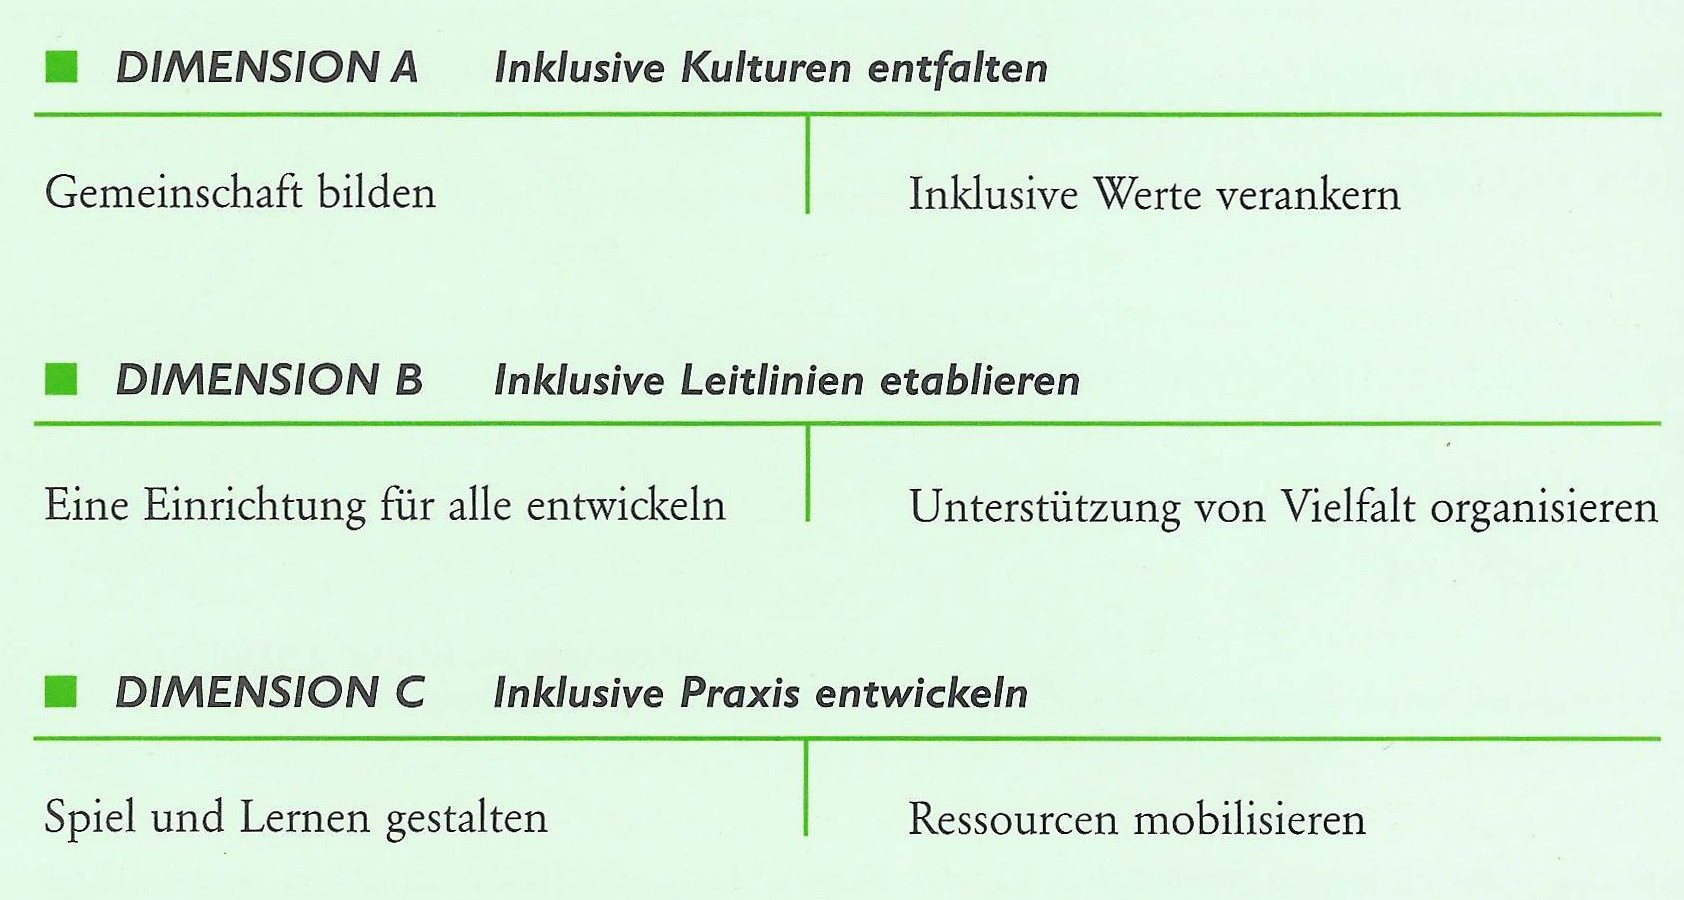
\includegraphics[width=0.8\textwidth]{bilder/planungsrahmen}
  \caption{Planungsrahmen}
\end{figure}

\paragraph{Inhaltsstruktur des Index} Den Planungsrahmen bilden dabei laut der Autoren (2011, 20) drei Dimensionen, die jeweils in zwei Bereiche unterteilt werden (vgl. Tabelle in Abbildung~\ref{pic:planungsrahmen}). 
Diese weisen enge Wechselbezüge auf: Inklusive Kulturen (Dimension A) schafft ein Kindergarten, in dem er sich als sichere, akzeptierende, kooperative und anregende Gemeinschaft entwickelt und dieser inklusive Werte als gemeinsame Basis zugrunde legt. Das setzt voraus, dass allen neuen Kindern, Eltern und Mitarbeitern diese Werte vermittelt und gleichzeitig alle Entscheidungen an selbigen ausgerichtet werden.  
Dementsprechende inklusive Leitlinien (Dimension B) etabliert die Kindergartengemeinschaft, indem sie ihre Bedingungen und Regelungen überprüft und so gestaltet, dass alle Kinder in der Gemeinde aufgenommen und in ihrer Vielfalt unterstützt werden. Inklusive Praktiken (Dimension C) entwickelt der Kindergarten, indem er entsprechende Aktivitäten, Angebote und Lernarrangements bereitstellt und materielle und individuelle Ressourcen mobilisiert, in Bezug auf  die Kinder, die Leitungsgremien der Träger, die Eltern oder das sozialräumliche Umfeld, alles was Spiel, Lernen und Partizipation fördert, kann in Frage kommen.   

\begin{figure}
  \centering
  \label{pic:indexProzess}
  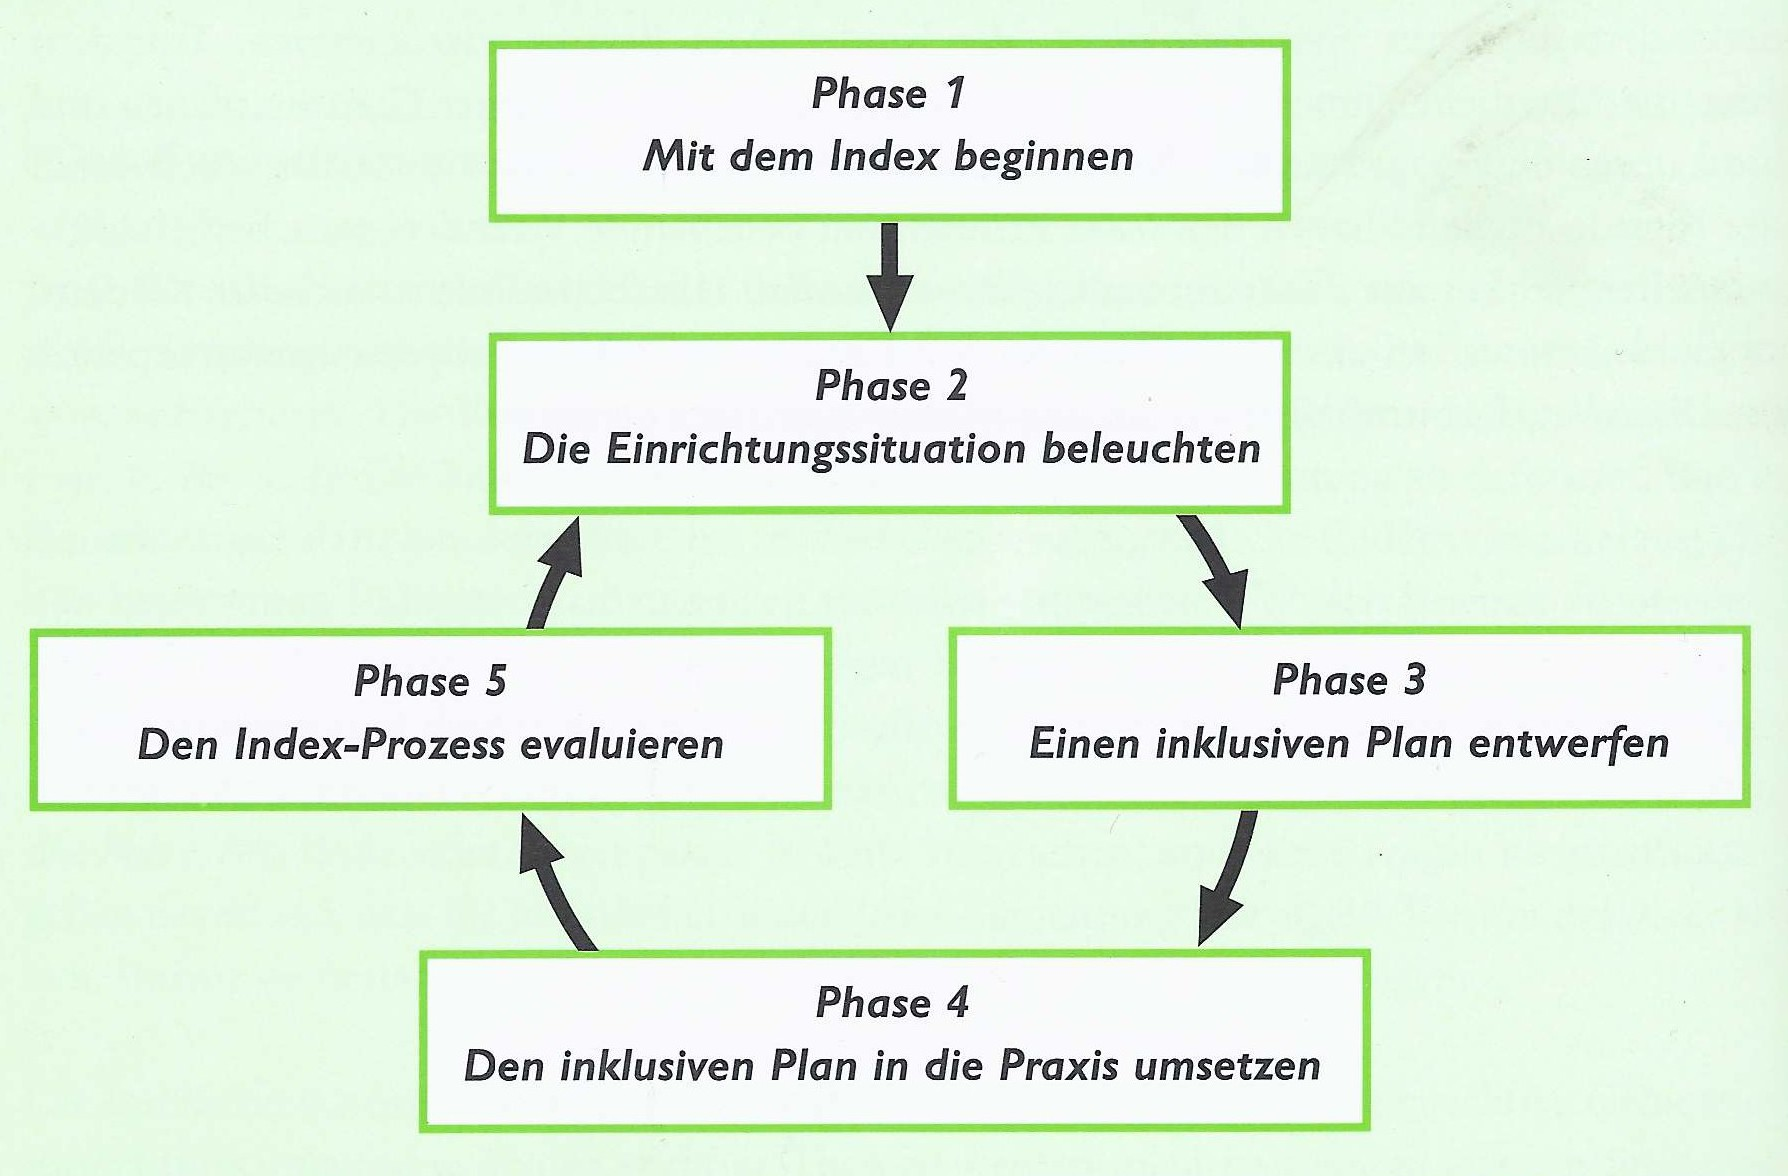
\includegraphics[width=0.8\textwidth]{bilder/indexProzess}
  \caption{Index-Prozess}
\end{figure}

\paragraph{Der Index-Prozess}

Der Index-Prozess selbst zeigt ein Vorgehen in fünf Phasen (vgl. Abbildung~\ref{pic:indexProzess}), was als Orientierung zu betrachten ist, das heißt, dass angepasst an die Situation der Einrichtung gegebenenfalls ein anderes Vorgehen als hilfreicher empfunden wird.  
In Phase 1 des Index-Prozesses „Mit dem Index beginnen“ (Booth et al. 2011, 32) soll das Index-Team gebildet werden, welches sich zunächst mit den Materialien und ihrer Verwendung vertraut macht. Das Index-Team leitet die internen Entwicklungsprozesse der Einrichtung und sollte deshalb strategisch sinnvoll gewählt werden, so dass durch die Personengruppen gute  Voraussetzungen geschaffen werden, die Einrichtung in Richtung Inklusion zu lenken. Auch eine als „kritischer Freund“ bezeichnete Person von außerhalb, jemand, der die Einrichtung kennt, Vertrauen genießt, im Idealfall auch den Index kennt oder noch besser damit arbeitet, kann sich als Moderator einbringen und dem Team helfen, mit kritischen Fragen umzugehen. Seine Funktion ist vielfältig und wird durch den Bedarf ermittelt. Phase 1 dient dazu miteinander und mit den Materialien, den Indikatoren und Fragen, vertraut zu werden, um ein Bewusstsein für den Index zu bekommen. Das setzt auch voraus, dass ein Austausch über das Selbstverständnis von Inklusion stattfindet.  
In Phase 2 „Die Einrichtungssituation beleuchten“ (ebd.) erfolgt eine intensive Bestandsaufnahme. Dabei wird unter Beteiligung der  unterschiedlichen Personengruppen, den Mitarbeitern, der Leitung, der Trägervertretung und den Kindern, zu einem Austausch angeregt, um das Wissen, die Ideen und die Prioritäten möglichst aller Beteiligten herauszufinden. Hierfür sind Indikatoren und Fragebögen für Eltern, Kinder und Mitarbeiter vorgesehen (vgl.~127-137). Je intensiver die Bestandsaufnahme erfolgt und je stärker die Gruppen beteiligt sind, desto qualifizierter und nachhaltiger dürfte die Planung der nächsten Schritte gelingen. 
Phase 3 sieht demnach, „einen inklusiven Plan [zu] entwerfen“ (ebd.), die zuvor erarbeiteten Prioritäten werden mit Hilfe der Handreichung „Prioritäten für die Entwicklung“ (Booth et. al. 2011, 129) zusammengetragen, überarbeitet und letztlich in den Entwicklungsplan und das Konzept eingefügt.
In Phase 4 „Den inklusiven Plan in die Praxis umsetzen“ (Booth et. al. 2011, 32) werden die beschlossenen Prioritäten in die Praxis umgesetzt.  
Booth et. al. (2011, 61) zeigen anhand eines exemplarischen Kindergartens, was Phase 4 zum Inhalt hat: „Wir entschlossen uns, die Leitlinien zum ,sonderpädagogischen Förderbedarf' in Leitlinien zur Inklusion zu ändern. Wir haben jetzt eine ,Inklusionsbeauftragte' statt einer 'Beauftragten für sonderpädagogischen Förderbedarf', aber wichtiger ist, dass sich die Tätigkeit geändert hat, so dass die Bedürfnisse aller Kinder berücksichtigt werden.“   
Es wird empfohlen die Fortschritte zu dokumentieren, so dass diese in Phase 5 „Den Index-Prozess evaluieren“ (ebd.) herangezogen werden können. Im letzten Schritt wird die Arbeit mit dem Index evaluiert, das heißt wiederum, der Prozess wird reflektiert und dokumentiert. Zur Orientierung werden Fragen aufgelistet (2011, 67), zum Beispiel wie gut hat das Index-Team funktioniert oder in welchem Ausmaß gab es ein steigendes Engagement für inklusive Arbeitsweisen? Nach der Evaluation ist im Bemühen um Nachhaltigkeit mit dem Index Prozess fortzusetzen. 
  
Diese fünf Schritte selbst sind so angelegt, dass sie Inklusion befördern und zu dauerhaften Verbesserungen beitragen.

\chapter{Aktueller Forschungsstand}\label{Forschung}
Um den Forschungsstand differenziert zu erheben, erschien es sinnvoll sowohl einschlägige Dokumentationen und Diskussionsforen für Forschung heranzuziehen als auch in der Literatur und im Internet gezielt nach Forschungsstudien mit Hilfe der Datenbank der Universität Freiburg zu Inklusion und angrenzenden Themenbereichen wie Integration oder Partizipation im Kontext Kindergarten zu suchen.

Bislang wurden nur sehr wenige Forschungsstudien zu Themen wie Inklusion und Integration oder auch Partizipation im Kontext Kindergarten veröffentlicht, vor allem wenige breit angelegte, die auf einer hinreichend großen Datenbasis basieren. Der Grund ist darin zu suchen, dass Deutschland in Bezug auf die Systemveränderungen hinsichtlich inklusiver Erziehungs- und Bildungsarbeit noch ganz am Anfang steht. Auch wenn es laut Heimlich und Behr (2006, 204) Schwerpunkteinrichtungen mit langjährigen Erfahrungen der gemeinsamen Erziehung und Bildung gibt, bilden diese doch die Ausnahme.  
Zudem nimmt die frühpädagogische Forschung an sich in Deutschland eine vergleichsweise untergeordnete Rolle ein. 
Tietze et al. (2012, 3) machen darauf aufmerksam, dass es in Deutschland – anders als im anglo-amerikanischen Kontext – bislang keine übergreifend angelegten Untersuchungen zur pädagogischen Qualität in den verschiedenen Betreuungsformen, zu ihren Voraussetzungen wie auch zu Zusammenhängen mit dem Bildungs- und Entwicklungsstand der Kinder gibt. Ebenso wenig verfügten Träger, Jugendamt oder Ministerium über Daten der pädagogischen Qualität von Kindertageseinrichtungen im eigenen Verantwortungsbereich, was bedeutet, dass elementare Daten für die Qualitätssteuerung fehlen.

Als Antwort auf diesen Mangel und um zentrale Fragen
hinsichtlich der Qualität in unserem Früherziehungssystem zu
untersuchen, wurde die breit angelegte NUBBEK-Studie durchgeführt, deren Ergebnisse im April 2012 erstmals einer ausgewählten Fachöffentlichkeit vorgestellt wurden. 
Der Fokus dieser Studie lag nicht auf Inklusion, somit sind die Ergebnisse für die Bachelorthesis nur insofern relevant, als dass sie zeigen, wie sich die frühe Bildung und Erziehung für Kinder mit Migrationshintergrund darstellt. 
Laut Tietze et al. (2012, 13 ff.) werden Kinder mit Migrationshintergrund vergleichsweise spät in öffentliche Einrichtungen  gegeben, weshalb ihnen bildungsrelevante Erfahrungen, vor allem im Hinblick auf den Erwerb der deutschen Sprache, verloren gehen. Dem frühzeitigen Besuch der Tageseinrichtung wird eine kompensatorische Wirkung im Hinblick auf den Spracherwerb zugeschrieben. Weiterhin haben die Ergebnisse gezeigt, dass Gruppen mit einem hohen Anteil an Kindern mit Migrationshintergrund eine besonders niedrige Prozessqualität aufweisen. Das heißt, dass gerade diejenigen Gruppen, für die eine qualitativ hochwertige Betreuung und eine optimale Förderung vor Schulbeginn besonders wichtig sind, geringere Chancen dazu haben.
Lösungen werden in hoch qualifiziertem Personal und einem verbesserten
Erzieher-Kind-Schlüssel gesehen. 
Die Qualität der Prozesse fällt nicht nur innerhalb der Kindergartengruppe schlechter aus, sondern ebenfalls innerhalb der zugewanderten Familien, was sich durch schlechter Voraussetzungen, wie  geringeres Einkommen und geringeren Bildungsstands, erklären lässt. 
Kinder mit Migrationshintergrund zeigen wie erwartet geringere Kompetenzen in der deutschen Sprache, da die meisten unter ihnen zweisprachig aufwachsen, schneiden jedoch in den sprachunabhängigen Kompetenzen zum Teil besser ab als ihre Altersgenossen ohne Migrationshintergrund.
  
Der fehlende Konsens über die Bedeutung des Inklusionsbegriffs hat laut Görannson (2010, 20 f.) Konsequenzen auf die Forschung, da das Verständnis von Inklusion darüber bestimmt, wie über Inklusion geforscht wird. So gibt es verschiedene Fragestellungen, die für die Forschung von Interesse sein könnten. Liegt dem Forschungsinteresse das Verständnis von Inklusion als undifferenzierte Gleichsetzung von Integration zugrunde, impliziert dieses nach Görannson (2010, 21) die Forschungsfrage, ob inklusive beziehungsweise heterogene Gruppen soziale Beziehungen unterstützen und ein gutes Lernfeld für jedes Kind ermöglichen. Setzt das Inklusionsverständnis die Notwendigkeit der individuellen Anleitung und Unterstützung des Kindes voraus, um dessen Teilhabe zu erhöhen, so lässt sich laut Serrano und Afonso (2010, 44) diese Dimension an dem Grad messen, in dem sich Kinder aktiv an bedeutungsvollen Lernaktivitäten beteiligen, das heißt anhand des zeitlichen Umfangs, in dem ein Kind in einer seiner Entwicklung und dem Zusammenhang gemäßen Art und Weise -- also auf individuellem Kompetenzniveau -- mit seinem Umfeld interagiert.
Inklusion, verstanden als langfristiger Prozess der Umstrukturierung, impliziert das Forschungsinteresse einen Beitrag zur Herstellung inklusiver Bildungs- und Erziehunseinrichtungen zu leisten sowie mit Hilfe von empirischer Begleitforschung die Umsetzung in der Praxis kritisch zu überprüfen, wodurch Inklusion wissenschaftlich fundiert und weiterentwickelt werden kann.

Ein Beitrag zur Herstellung inklusiver Kindertageseinrichtungen ist durch das Projekt QUINTE (Qualitätsstandards für die Integrationsentwicklung in Kindergärten der Landeshauptstadt München) unter der Federführung von Ulrich Heimlich erfolgt. An diesem Forschungsprojekt beteiligten sich laut Heimlich und Behr (2006, 200) elf Kindergärten der Stadt München, die in dem Jahr 2002/2003 bereits integrativ arbeiteten. Als Ergebnis dieses Projekts sind 26 Qualitätsstandards als Orientierungsmöglichkeiten für die Integration der frühen Kindheit entwickelt worden, die nun in die Praxis der Kindertageseinrichtungen implementiert und der Entwicklung weiterer inklusiver Einrichtungen zugrunde gelegt werden können. 
Darüber hinaus zeigen die Ergebnisse, dass die integrative Qualität zum gegenwärtigen Zeitpunkt gut entwickelt ist und dass diese Einrichtungen eine größere Zufriedenheit unter den Eltern und Mitarbeitern vorweisen können als Einrichtungen, die nicht integrativ arbeiten. Entsprechend des inklusiven Verständnisses können als Mängel lediglich die Erreichbarkeit der unterschiedlichen Räume im Sinne der Barrierefreiheit und die Umsetzung der integrativen Therapien genannt werden.  

Inklusive Erziehungs- und Bildungsarbeit kann auch durch die Anwendung des Index für Inklusion unterstützt werden. Haefke und Mattke (2011, 134 f.) weisen daraufhin, dass selbige Handreichung im deutschsprachigen Raum jedoch kaum Anwendung findet. Ihre Recherche hat ergeben, dass dieses Hilfsmittel bisher lediglich in Kindertagesstätten in Köln und in zwei Kindertagesstätten in Baden-Württemberg sowie in dem sich auf eine ganze Gemeinde beziehenden österreichischen Inklusionsprojekt in Wiener Neudorf eingesetzt wurde. Die Autoren beschreiben die Erprobung des Index in einer norddeutschen Regelkindertagesstätte und seinen Erfolg auf verschiedenen Ebenen, insbesondere in der beruflichen Kooperation der Erzieherinnen sowie in der Vernetzung innerhalb des Gemeinwesens. Die Vernetzung mit dem Träger konnte mit Hilfe einer Trägervertreterin in das Index-Team deutlich erhöht werden. Die Erfahrung im Team zeigt, dass der Index für Inklusion zunächst als größere Hürde empfunden wurde, sich im Ergebnis jedoch als geeignetes Handwerkszeug erwies. Eine beratende Begleitung von außen wurde als hilfreich empfunden, um mit diesem Hilfsmittel vertraut zu werden. Der Veränderungsprozess war von großer motivierender Wirkung für das Team, da der Index für Inklusion einen Ansatz zur Verbesserung fern von negativ konnotierten Qualitäten wie Überprüfung, Wettbewerb und Versagensangst bereithält.

Einige Veröffentlichungen befassen sich mit der Frage der Beteiligung von Kindern mit einer Behinderung an der Kindergruppe. Hierbei wird die Frage tangiert, ob heterogene Gruppen soziale Beziehungen der Kinder untereinander unterstützen. Kreuzer (2011, 23-31) gibt einen Überblick über die Ergebnisse der im Zeitraum von 1980 bis 1995 in Deutschland durchgeführten Modellprojekte zur Integration. Gemeinsam ist diesen Arbeiten, dass sie bedingt durch die damals üblichen Einzelintegrationsmaßnahmen der Einzelfallforschung zuzuordnen sind, weshalb sie nicht repräsentativ sind, aber insofern als relevant angesehen werden, als dass sie als Erfahrungswerte in die Weiterentwicklung hin zu Inklusion einfließen können. Gleichzeitig verdeutlichen die Ergebnisse, wo Deutschland zu welcher Zeit bezüglich der Integrationsentwicklung stand. Fritzsche, Schastock und Schöler (2005, 80) weisen daraufhin, dass diese Modellprojekte weitestgehend ohne Erfahrungswerte und ohne eine Qualifizierung der Erzieherinnen für den Umgang mit behinderten Kindern auskommen mussten. 

Auch die in den Untersuchungsergebnissen verwendeten Kategorien Behinderung und Nicht-Behinderung zeigen ein Integrationsverständnis, das gemessen an dem leitenden Inklusionsverständnis dieser Arbeit als überholt gelten kann. Kreuzer (2011, 30) kommt zu dem Schluss, dass „solche Generalisierung bezogen auf die Beteiligung im Gruppenalltag nur von geringer Trennschärfe sind“ (Kreuzer 2011, 30) und wenn die festgestellten Unterschiede nur an der Behinderung festgemacht werden, stigmatisierenden Charakter haben. Alternativ dazu und im Sinne von Inklusion würden die wahrnehmbaren Unterschiede an allgemeinen Kriterien wie Alter, Geschlecht, Verhaltensweisen, Basisfertigkeiten entlang interpretiert werden, so dass die Kinder in erster Linie als Mitglieder der jeweiligen Peergruppe verstanden werden. Sowohl Kreuzer als auch Fritzsche et al. (2005, 82) beschreiben den Begriff der Behinderung für die Beschreibung eines Zustandes innerhalb des Kindergartensystems als ungeeignet. 

Folgend werden einige Forschungsergebnisse von Kreuzer (2011, 26-31) zusammengefasst.

\begin{itemize}
\item Die Ergebnisse aus der Kasseler Untersuchung von dem Ehepaar Kniel (1984) zeigen, dass behinderte Kinder häufiger als Vergleichskinder alleine oder gemeinsam mit einer oder bei einer Erzieherin spielen sowie dass sie seltener die aktive Rolle im Zusammenspiel einnehmen. Beobachtet werden konnte, dass behinderte Kinder mehr als die Hälfte der Zeit im Parallelspiel verbringen, das heißt, dass sie die gleiche oder eine ähnliche Tätigkeit ausführen, sich aber nicht in wechselseitige Interaktion begeben, etwa 30\,\% der Zeit allein und nur knapp 20\,\% in Kooperation miteinander verbringen. Darüber hinaus konnte gezeigt werden, dass behinderten Kinder ihre Wünsche und Bitten zu 70\,\% an Erwachsene richten, während Vergleichskindern nur zu 40\,\% Erwachsene adressieren. Insbesondere stark motorisch eingeschränkte Kinder fallen durch ihre starke Erwachsenenorientierung ins Auge. Ihre Situation in Konflikten entspricht der anderer Kinder, ebenso erleben sie gleich häufig eine ablehnende Reaktion auf auf ihre Anfragen.

\item Im Dortmunder Modellprojekt von Heimlich (1993) konnte beobachtet werden, dass behinderte Kinder eine deutlich verlängerte Eingewöhnungs- und Adaptions\-phase zeigen. Heimlich geht davon aus, dass „die Hauptschwierigkeiten des Integrationsprozesses im ersten Aufenthaltsjahr im Kindergarten zu bewältigen sind“ (Heimlich in Kreuzer 2011, 27) und die Erzieherinnen für die Gestaltung sozialer Kontakte und die Überwindung möglicher Schwierigkeiten in der Kontaktanbahnung besondere Kenntnisse benötigen.

\item Fichtner und Timmann (1995) schreiben in ihrem Abschlussbericht des niedersächsischen Erprobungsprogramms \emph{Gemeinsame Erziehung}, dass nach Wegen gesucht werden muss, verstärkt Spiel- und Lernprozesse der Kinder untereinander anzuregen. Eine direkte Beteiligung der Fachkräfte würde die Interaktionen jedoch hemmen, da sie sich negativ auf die Selbsttätigkeit auswirkt. Eine Ausnahme bilden schwer- und schwerstbehinderte Kinder, für sie sei die anregende Beteiligung zu Interaktionen von Seite der pädagogischen Fachkraft wichtig. 

\item Klein, Kreie, Kron und Reiser (1984) beobachteten im Laufe ihrer auf zwei Jahre angelegten Studie, dass wahrnehmungs- und bewegungsbeeinträchtigte Kinder in integrativen Gruppen „Bezugspunkte für Wärme und Zärtlichkeit“ (Klein et al. in Kreuzer 2011, 28) darstellen, weil der Zugang und die Versorgung dieser Kinder vermehrt unter Einbezug von Körperkontakt geschieht. Der Alltag in integrativen Gruppen lässt sich im Vergleich zu Regelgruppen als insgesamt körperorientierter beschreiben. Kritisch wird von der Autorin der vorliegenden Arbeit angemerkt, dass Körperkontakt eine Antwort auf kindliche Bedürfnisse nach Nähe, emotionaler Sicherheit und Unterstützung ist, sofern die Autonomiebestrebungen des Kindes sensibel wahrgenommen und durch zu viel Unterstützung nicht behindert werden.  

\item die Ergebnisse der Beobachtungen eines Jungen mit einer schweren spastischen Bewegungseinschränkung von Fritzsche et al. (2005, 106 f.)  zeigen, dass sich die Beschäftigungsangebote der Erzieherin für die ganze Gruppe stark an den Bedürfnissen der nicht-behinderten Kinder orientieren, mit dem Ergebnis, dass für das spastische Kind eine Extrabeschäftigung gefunden werden muss oder es so umfangreiche Hilfe bei der Ausführung der Aufgabe benötigt, dass nicht mehr von Selbsttätigkeit gesprochen werden kann. Die pädagogische Arbeit ist hier noch sehr durch die Orientierung am Ergebnis geprägt, statt dass im Mittelpunkt das gemeinsame Tun und soziale Miteinander steht. In einer Befragung der Erzieherinnen begründen diese ihre Arbeitsweise, indem sie anführen, dass die Eltern solche Ergebnisse sehen wollen würden.

\end{itemize}